\documentclass[12pt,paper=a4]{report}
%Nepieciešamās pakotnes---------------------------------------------------------------------------------------------
%Valodu atbalsts
\usepackage{polyglossia}
\usepackage{url}
%Atkāpes pirmajām rindiņām
\usepackage{indentfirst}
%Atstarpes starp rindiņām
\usepackage{setspace}
%Virsrakstu noformējumam
\usepackage{titlesec}
%Attēlu importēšanai
\usepackage{graphicx}
%Vajadzēs saliktus attēlus
\usepackage{subcaption}
%Nodefinē attālumus no malām
\usepackage[a4paper, lmargin=3.5cm,rmargin=2cm,tmargin=2cm, bmargin=2cm]{geometry}
%Matlab koda importēšanai
\usepackage[framed,numbered,autolinebreaks,useliterate]{mcode}
%Pseidokoda rakstīšanai
\usepackage{algorithm}
\usepackage{algorithmic}
%Tabulu šūnu iekrāsošanai
\usepackage{xcolor,colortbl}
%Apjomīgām tabulām
\usepackage{longtable}
%Numerācijai lappuses labajā pusē
\usepackage{fancyhdr}
%Literatūras saraksta veidošanai
\usepackage{natbib}
%Garas formulas
\usepackage{amsmath}
%Lai varetu ievietot lapu landscape
\usepackage{lscape}
%Noformējuma parametri---------------------------------------------------------------------------------------------
%Nodefinējam valodas
\setdefaultlanguage{latvian}
\setotherlanguages{english,russian}




%Fonts un atstarpe starp rindām
\setmainfont{Times New Roman}
\newfontfamily\russianfont{Times New Roman}
\fontsize{12pt}{1.5}
\onehalfspacing
%Rindiņas pirmā atkāpe
\setlength{\parindent}{1.27cm}
%Apakšmape bildēm
\graphicspath{{./images/}}
%Krāsa dažādiem ieēnojumiem
%\definecolor{shadecolor}{rgb}{0.75, 0.85, 0.38}
%Virsrakstu formatējums
\newfontfamily\sffamily{Times New Roman}
\newfontfamily\russianfont{Times New Roman}
%\titleformat{\chapter}{\large\centering\sffamily\bfseries}{\thechapter}{0pc}{}
%{\chaptertitlename\ \thechapter}{20pt}{\Huge}
\titleformat{\chapter}
  {\centering\sffamily\fontsize{16}{16}\bfseries}{\thechapter}{0pc}{}
\titleformat{\section}{\sffamily\fontsize{14}{14}\bfseries}{\thesection}{0pc}{}
\titleformat{\subsection}{\sffamily\fontsize{12}{12}\bfseries}{\thesubsection}{0pc}{}
\titlespacing*{\chapter}{0pt}{0pt}{10pt} 
\titlespacing*{\section}{0pt}{0pt}{5pt} 
\titlespacing*{\subsection}{0pt}{0pt}{5pt} 
    
%Nodefinējam objektu numerācijas noteikumus
\def\thechapter      {\arabic{chapter}.}
\def\thesection      {\ifx\chapter\undefined{\arabic{section}.}\else  {\thechapter\arabic{section}. }\fi}
\def\thesubsection   {\thesection\arabic{subsection}. }
\def\thesubsubsection{\thesubsection\arabic{subsubsection}. }


\renewcommand{\thefigure}{\arabic{chapter}.\arabic{figure}.}
\renewcommand{\theequation}{\thechapter \arabic{equation}.}
\renewcommand{\thetable}{\thechapter \arabic{table}.}
%Attelu un tabulu nosaukumi
\captionsetup[figure] {labelformat=default,labelsep=space}
\captionsetup[table] {labelformat=simple,labelsep=space}
\renewcommand{\figurename}{att.}
%\renewcommand{\thefigure} {\arabic{\figure}}
%\renewcommand{\fnum@figure}{\thefigure ~S \figurename}
\renewcommand{\tablename}{tabula}
%\makeatletter
%\renewcommand{\fnum@figure}{}
%\makeatother
%Teksta nodaļu fiksētie nosaukumi
 
\addto\captionslatvian{
\renewcommand\bibname{Izmantotās literatūras un avotu saraksts}
\renewcommand{\contentsname}{Saturs}
}

%Nodefine krasu
\definecolor{Gray}{gray}{0.85}
\definecolor{Green}{rgb}{0,1,0}

%Numeracija

\pagestyle{fancy}

\fancyhf{}
\renewcommand{\headrulewidth}{0pt} 
\renewcommand{\footrulewidth}{0pt}
\fancyfoot[R]{\thepage}
\fancypagestyle{plain}{%
  %\fancyhf{}%
  \fancyfoot[R]{\thepage}%
}
%Pārnesumiem - ļauj tiasīt lielākas starpas
\hyphenpenalty=5000
%% Atraitņrindiņas un bāreņrindiņas ( widow orphan) vadība
\clubpenalty10000
\widowpenalty10000
% Apakšsvītrām
\usepackage{underscore}

\begin{document}
\begin{titlepage}
\begin{center}
\textbf{VENTSPILS AUGSTSKOLA\\
INFORMĀCIJAS TEHNOLOĢIJU FAKULTĀTE}\\
\vspace{1.2cm}
\textbf{MAĢISTRA DARBS}\\
\vspace{1.4cm}{\LARGE \textbf{Zemes pārseguma klasifikācija, izmantojot tālizpētes datus.}}\\\vspace{1cm}
\begin{tabular}{@{}r@{}l@{}}
\parbox[c]{0.4\textwidth}{Autors:}&
\parbox[t]{0.6\textwidth}{
Ventspils Augstskolas\\
Informācijas tehnoloģiju fakultātes\\
maģistra studiju programmas "Datorzinātnes" \\
2. kursa studente\\
Katrīna Zvaigzne \\
Matr. Nr. 15080010
\vspace{0.7em}\\
\mbox{}
\hrulefill
\vspace{-0.4em}\\
{\scriptsize(paraksts)}
\vspace{1.2cm}} \\
\parbox[c]{0.4\textwidth}{Fakultātes dekāns:}&
\parbox[t]{0.6\textwidth}{doc. Dr. phys. Māris Ēlerts 
\vspace{.7em}\\
\mbox{}
\hrulefill
\vspace{-0.4em}\\
{\scriptsize(paraksts)}
\vspace{1.2cm}} \\
%-------------------------------------------------------------------------
\parbox[c]{0.4\textwidth}{Zinātniskā vadītāja:}&
\parbox[t]{0.6\textwidth}{Mg.sc.comp. Linda Gulbe 
\vspace{.7em}\\
\mbox{}
\hrulefill
\vspace{-0.4em}\\
{\scriptsize(paraksts)}
\vspace{1.2cm}} \\
%----------------------------------------------------------------------------------
\parbox[c]{0.4\textwidth}{Recenzents:} & %\vspace{.7em}\\
\parbox[t]{0.6\textwidth}{
 \hspace{3cm} \\
\mbox{}\hrulefill\vspace{-0.4em}\\
{\scriptsize(Ieņemamais amats, zinātniskais nosaukums,
vārds, uzvārds)}\vspace{2em}

\mbox{}\hrulefill\vspace{-0.4em}\\
{\scriptsize(paraksts)}\vspace{2em}} \\
\end{tabular}
\vfill
Ventspils, 2017
\end{center}
\end{titlepage}
\setcounter{page}{2}

%Vieta anotācijām---------------------------------------------------------------------------
\chapter*{ANOTĀCIJA}
\textbf{Darba nosaukums:} Zemes pārseguma klasifikācija, izmantojot tālizpētes datus.\par
\textbf{Darba autors:} Katrīna Zvaigzne\par
\textbf{Darba vadītājs:} mg. sc. comp. Linda Gulbe\par
\textbf{Darba apjoms:} 48 lpp., 2 tabulas, 24 attēli, 28 bibliogrāfiskās norādes.\par
\textbf{Atslēgas vārdi:} ORTOFOTOKARTES, ATTĒLU SEGMENTĀCIJA, VADĪTĀ KLASIFIKĀCIJA, DZIĻĀS APMĀCĪBAS NEIRONU TĪKLI. \\ \par
Maģistra darbā ir apskatīta attēlu segmentācijas metode JSEG un vairākas citas eksistējošas metodes krāsu attēlu segmentācijā. Izanalizēti šo metožu trūkumi un priekšrocības salīdzinoši ar JSEG attēlu segmentācijas metodi. Papildus analizēta arī JSEG iekļautā segmentēto reģionu apvienošanas metode un atrastas alternatīvas tās aizvietošanai.\par
Autore izstrādājusi darbplūsmas ne tikai ortofotokaršu segmentēšanā izmantojot JSEG, bet arī implementējusi atrastās alternatīvas reģionu klasificēšanā. Lai noteiktu, kura no klasifikācijas metodēm sniedz labākus rezultātus, veikta klasificēto reģionu validācija gan klasifikācijai, izmantojot k-tuvāko kaimiņu metodi, gan, izmantojot neironu tīklus.\par
Maģistra darba rezultātā veikta ortofotokartes segmentēšana izmantojot attēlu segmentēšanas algoritmu JSEG, izpētītas klasifikācijas metodes zemes pārseguma tipu noteikšanai augstas telpiskās izšķirtspējas multispektrālajos datos un izstrādātas darbplūsmas metožu pielietošanai. 
\chapter*{ABSTRACT}
\textbf{Title: }Land cover classification using remote sensing data. \par
\textbf{Author: }Katrina Zvaigzne \par
\textbf{Supervisor: }mg. sc. comp. Linda Gulbe \par
\textbf{Volume: }48 pages, 2 tables, 24 images, 28 citations. \par
\textbf{Key words: }ORTHOPHOTOMAP, IMAGE SEGMENTATION, SUPERVISED CLASSIFICATION, DEEP LEARNING NEURAL NETWORKS. \\ \par
This master`s thesis examines JSEG and a number of other color image segmentation methods. An analysis on these methods was done and pros and cons of each of those methods was found. Additional analyzes also included JSEG segmented region merging method and found alternatives. \par
The author created a workflow not only for orthophotomap segmentation using JSEG but also implemented regional classification alternatives. To determine which of the classification methods gives better results, conducted classified region validation using the k-nearest neighbor method and using neural networks. \par
As a result of master`s thesis, orthophotomap segmentation was performed using JSEG, methods for segmented region classification into land cover types were researched and created workflows were applied.
%Saturs---------------------------------------------------------------------------------------
\tableofcontents
%Darba ievads bez numerācijas -------------------------------------------------------------------
\chapter*{Ievads}
\addcontentsline{toc}{chapter}{Ievads}
Zemes pārsegums apraksta Zemes virsmas fizisko pārklājumu un parasti to sagrupē tipos atkarībā no  nepieciešamās informācijas, piemēram, zemes pārsegumu var iedalīt lauksaimniecības platībās, ūdeņos, mežos, ceļos un apdzīvotās teritorijās. Zemes pārseguma tipu izšķiršana ir nozīmīga, lai būtu iespējams noteikt izmaiņas, ko izraisījušas kādas pārmaiņas dabā. \cite{landCoverTypes1976}\par 
Piemēram, zemes pārseguma tipu kartes ir noderīgas gan pirms ugunsgrēkiem, lai modelētu potenciālo risku, gan ugunsgrēka laikā, lai atbalstītu drošības personālu ugunsgrēku apkarošanā un evakuācijas organizēšanā, gan arī pēc ugunsgrēka, lai mazinātu ugunsgrēka ietekmi uz dabu. Vēl ir nozīmīgi izšķirt apdzīvotas teritorijas no veģetācijas plašā ģeogrāfiskā apgabalā, lai, balstoties uz ēku atrašanās vietām attiecībā pret viegli uzliesmojošām teritorijām, būtu iespējams novērst zaudējumus, kas var rasties savvaļas ugunsgrēku dēļ. \cite{cleve2008classification}\par
Nepārtrauktā vides mainība ir viens no iemesliem, kādēļ zemes pārseguma tipu kartes ātri noveco un kļūst nederīgas. Aktuāla informācija par interesējošo reģionu ir nepieciešama lielu zemes platību īpašniekiem un apsaimniekotājiem, kam fiziska platību apzināšana ne vienmēr ir un arī patērē ļoti daudz laika. Līdzīga situācija ir mākleriem un dažādiem īpašumu pārpircējiem, kam ne vienmēr ir interese fiziski un padziļināti apsekot katru nekustamo īpašumu. \par
Ortofotokartes sadalīšana zemes pārseguma tipos notiek divos soļos - attēla segmentēšana un segmentācijas rezultātu klasifikācija zemes pārseguma tipos. Džollija un Gupta savā pētījumā "\textit{Color and Texture Fusion: Application to Aerial Image Segmentation and GIS Updating} \cite{jolly1996color}" krāsu aerofotogrāfiju segmentēšanu veic, izmantojot maksimālās ticamības segmentēšanu (angl. \textit{maximum likelihood segmentation}). Lai arī šī metode sniedz labus rezultātus, tās ierobežojumi saistāmi ar spēju labi segmentēt tikai viendabīgas tekstūras vai krāsas attēlus. \cite{jolly1996color} \par
Klīvs un citi savā pētījumā "\textit{Classification of the wildland–urban interface: A comparison of pixel- and object-based classifications using high-resolution aerial photography} \cite{cleve2008classification}" veic zemes pārseguma tipu klasifikāciju, izmantojot divas metodes. Pirmā pieeja ir balstīta uz atsevišķu pikseļu klasifikāciju, izmantojot \textit{ISODATA} nevadītās klasifikācijas metodi, bet otrā uz atsevišķu segmentētu reģionu klasifikāciju, izmantojot \textit{fuzzy} un \textit{tuvāko kaimiņu} vadītās klasifikācijas metodes. Otrajā pieejā aerofotogrāfijas segmentēšana notiek, izmantojot aplikāciju \textit{Definiens eCognition}. \cite{cleve2008classification} \par
Attēlu segmentēšana ir nozīmīga tālizpētes, attēlu analīzes un tēlu pazīšanas (LZA, angl. \textit{pattern recognition}) daļa. Tieši no segmentācijas rezultātiem iespējams iegūt nozīmīgu informāciju par interesējošiem reģioniem vai objektiem attēlā, kas noder turpmākai attēlu analīzei.\cite{4satImSegm2012} \par 
Tā kā zemes pārsegums ir ļoti dažāds kā krāsas, tā tekstūras ziņā, bet lielākā daļa segmentēšanas algoritmu labi strādā ar homogēniem krāsu reģioniem vai tiem nepieciešami precīzi tekstūras novērtējumi, kas ne vienmēr ir viegli nosakāmi, nepieciešami automātiski segmentēšanas algoritmi, kas ir spējīgi tikt galā ar dažādiem scenārijiem attēlā.\cite{4satImSegm2012},\cite{1colImSegm1999},\cite{2unsupImSegm2001} \par
Kā risinājums vairākos literatūras avotos (\cite{4satImSegm2012}, \cite{1colImSegm1999}, \cite{2unsupImSegm2001}, \cite{6buildings2008}, \cite{5forest2007}) tiek piedāvāts JSEG algoritms ar vai bez dažādām modifikācijām. \par
Segmentācijas algoritmi, tajā skaitā JSEG, attēlā identificē krāsas un tekstūras ziņā līdzīgus reģionus. Nākamais solis pēc segmentācijas ir reģionu klasifikācija, kura identificē konkrētu reģiona zemes pārseguma tipu. Balstoties uz vairākos pētījumos pausto informāciju, ka ne vienmēr JSEG iekļautais apvienošanas algoritms veiksmīgi veic segmentēto reģionu apvienošanu jēgpilnās reģionu grupās, tika pieņemts lēmums apvienot JSEG segmentēšanas metodi ar vadītās klasifikācijas k-tuvāko kaimiņu (LZA (Latvijas Zinātņu Akadēmija), angl. \textit{k-nearest neighbors}) metodi un arī veikt klasifikāciju, izmantojot neironu tīklus. \par
Maģistra darba mērķis ir izpētīt klasifikācijas metodes zemes pārseguma tipu noteikšanai ļoti augstas telpiskās izšķirtspējas multispektrālajos datos un izstrādāt darbplūsmas metožu pielietošanai.\par Lai sasniegtu maģistra darba mērķi, tika izvirzīti sekojoši uzdevumi:
\begin{itemize}
\item veikt ortofotokartes segmentāciju, izmantojot JSEG segmentēšanas metodi;
\item JSEG segmentēšanas gaitā veikt tādu parametru, kā pudurošanas pēc vidējiem (LZA, angl. \textit{kmeans}) parametru \textit{k}, mazākā loga izmēra, ortofotokartes fragmenta izmēru testēšanu, lai iegūtu eksperimentāli labākos rezultātus;
\item izpētīt metodes ortofotokaršu segmentācijas rezultātu klasifikācijā;  
\item sagatavot parauga datus;
\item izveidot validācijas datu komplektu;
\item klasificēt segmentācijas rezultātā iegūtos reģionus, izmantojot k-tuvāko kaimiņu metodi, un veikt rezultātu validāciju;
\item klasificēt segmentācijas rezultātā iegūtos reģionus, izmantojot neironu tīklus, un veikt rezultātu validāciju;
\item salīdzināt abu klasifikācijas metožu rezultātus un veikt secinājumus.
\end{itemize}\par
Maģistra darbs sastāv no ievada, trīs nodaļām, secinājumiem un priekšlikumiem. Pirmajā nodaļā apskatīti izmantotie dati un pētāmais apgabals, kā arī definēts tālizpētes attēls un tā izšķirtspēju veidi. Otrajā nodaļā apskatīti risinājumi zemes pārseguma atpazīšanai augstas telpiskās izšķirtspējas multispektrālajos datos un izstrādātas darbplūsmas risinājumu pielietošanai. Trešajā nodaļā tiek veikta klasificēto segmentācijas rezultātu validēšana un apkopoti rezultāti.\par
Pētījums tika realizēts, izmantojot salīdzinājuma pētniecības (LZA, angl. \textit{comparative study}) un izmēģinājuma studijas metodes. Pētījumā tika veikta literatūras avotu analīze un pētījuma praktiskā daļa tika veikta, izmantojot programmatūras \textit{MatLab}, \textit{QGIS}, programmēšanas valodu \textit{Python} un bibliotēku \textit{TensorFlow}.

\chapter{Izmantotie dati un pētāmais apgabals}
\section{Tālizpētes dati, attēls un tā izšķirtspējas veidi}Tālizpēte dažādos literatūras avotos ir definēta atšķirīgi, tomēr visām definīcijām ir kopīga iezīme, ka tālizpēte ir informācijas ieguve no attāluma bez tieša kontakta ar pētāmo objektu. Šāda definīcija ir ļoti vispārīga un gadījumos, kad tālizpētes metodes tiek izmantotas, lai iegūtu vispārīgu informāciju par Zemes pārsegumu, definīcija tiek precizēta uz informācijas ieguvi, izmantojot atstaroto vai izstaroto elektromagnētisko enerģiju.\par
Kempbels un Vains savā grāmatā \textit{Introduction to Remote Sensing} definē: "Tālizpēte ir informācijas iegūšanas prakse par Zemes pārsegumu, izmantojot attēlus, kas iegūti no satelītu vai aero platformām, un, kuros reģistrēts Zemes virsmas izstarotais un/vai atstarotais elektromagnētiskais starojums (LZA, angl. \textit{electromagnetic radiation}) vienā vai vairākos elektromagnētiskā spektra reģionos \cite{IntrToRemSensing}."\par
\subsection{Attēls un tā izšķirtspējas veidi}
No tālizpētes definīcijas izriet, ka biežāk izmantotais datu formāts ir attēls. Attēls ir divdimensionāla funkcija \(f(x,y)\), kur \(x\) un \(y\) ir plaknes koordinātes, bet amplitūdu katrā punktā \((x,y)\) sauc par attēla intensitāti vai pelēkā līmeni šajā punktā. Attēla ieguvē nozīmīgi ir tādi divi procesi kā diskretizācija un digitalizācija. Diskretizācija praktiski ir signāla telpiska sadalīšana konkrēta skaita iedaļās, ko vispārīgā gadījumā nosaka pusvadītāju sensoru skaits. Digitalizācija ir signāla intensitātes sadalīšana galīgās vienībās. Piemēram, ienākošo signālu iespējams digitalizēt divās vienībās izmantojot 1 un 0, kur ar 1 apzīmē tuvāk baltam esošos toņus, bet ar 0 tumšos toņus. Lai informācija, kas iegūstama no attēla, tiktu kvalitatīvi reprezentēta, jāpievērš liela uzmanība informācijas nesēja - attēla kvalitātei. Tālizpētes attēlu kvalitāti iespējams raksturot, izmantojot četru veidu izšķirtspējas:
\begin{itemize}
\item Telpiskā izšķirtspēja - tā ir izšķirtspēja, kas bieži veido primāro asociāciju ar šo terminu. Telpiskā izšķirtspēja nosaka to, cik liels ir mazākais objekts, kurš ir saskatāms attēlā. Realitātē telpisko izšķirtspēju izsaka kā attēla pikseļa dabiskos izmērus dabā. Piemēram, ar telpisko izšķirtspēju viens metrs iespējams pat izšķirt automašīnas, koku vainagus vai pat dažādus dzīvniekus, bet ar telpisko izšķirtspēju 30 metri šādas detaļas saplūst ar apkārtējo vidi.
\item Spektrālā izšķirtspēja raksturo elektromagnētiskā spektra daļas platumu nanometros (vai mikrometros), kuru uztver sensors. Šo elektromagnētiskā starojuma daļu sauc arī par kanālu vai frekvenču joslu. Esot augstākai spektrālai izšķirtspējai, iespējams uztvert mazāku viļņa garumu diapazonu. Multispektrālie sensori ievāc katrai frekvenču joslai atsevišķu pelēko toņu attēlu. Apvienojot zilā, sarkanā, zaļā un tuvā infrasarkanajā joslā iegūtos attēlus, iegūst dabisko krāsu attēlu. 
\item Radiometriskā izšķirtspēja - kā jau iepriekš tika minēts, digitalizācija pārveido attēlu galīga skaita vienību toņos. Tieši šo toņu skaits arī ir radiometriskā izšķirtspēja un to raksturo bitu dziļums jeb skaitļa divi pakāpe, kas nepieciešama, lai iegūtu nepieciešamo toņu skaitu.
\item Temporālā izšķirtspēja nosaka to, cik bieži pieejami konkrētās ģeogrāfiskās vietas attēli. \cite{gonzalez2002digital}
\end{itemize}
\section{Izmantotie dati}Maģistra darbā izmantota Latvijas Ģeotelpiskās Informācijas Aģentūras (LĢIA) ortofotokarte. Ortofotokarte ir zemes virsmas attēls, kas izgatavots no aerofotogrāfijām un kam, izmantojot speciālas, šim mērķim paredzētas datorprogrammas, novērsti visi sagrozījumi, kas rodas fotografējot reljefa un citu faktoru ietekmē. \cite{lgia}\par
Aerofotogrāfijas, no kā iegūta ortofotokarte, fotografētas 5. ciklā 2013. gada jūnijā, izmantojot 4 lidojumus - 1. un 2. jūnijā, 21. jūnijā, 23. jūnijā un 30. jūnijā. Ortofotokartes ir pieejamas \textit{TIFF} formātā un tās ir piesaistītas LKS-92 TM koordinātu sistēmai. \cite{lgia2}\par 
Ortofotokarte (redzama \ref{fig:fullIm} attēlā) ir kvadrātiska ar izmēru 10 000 $\times$ 10 000 pikseļi, kas dabā aptver 16 $km^2$ lielu teritoriju jeb vienas dimensijas garums ir 4 kilometri. Ortofotokartes telpiskā izšķirtspēja ir 0,4 metri uz pikseli. Ortofotokartes spektrālā izšķirtspēja ir redzamās gaismas RGB joslas. \par
\begin{figure}[h]
\centering
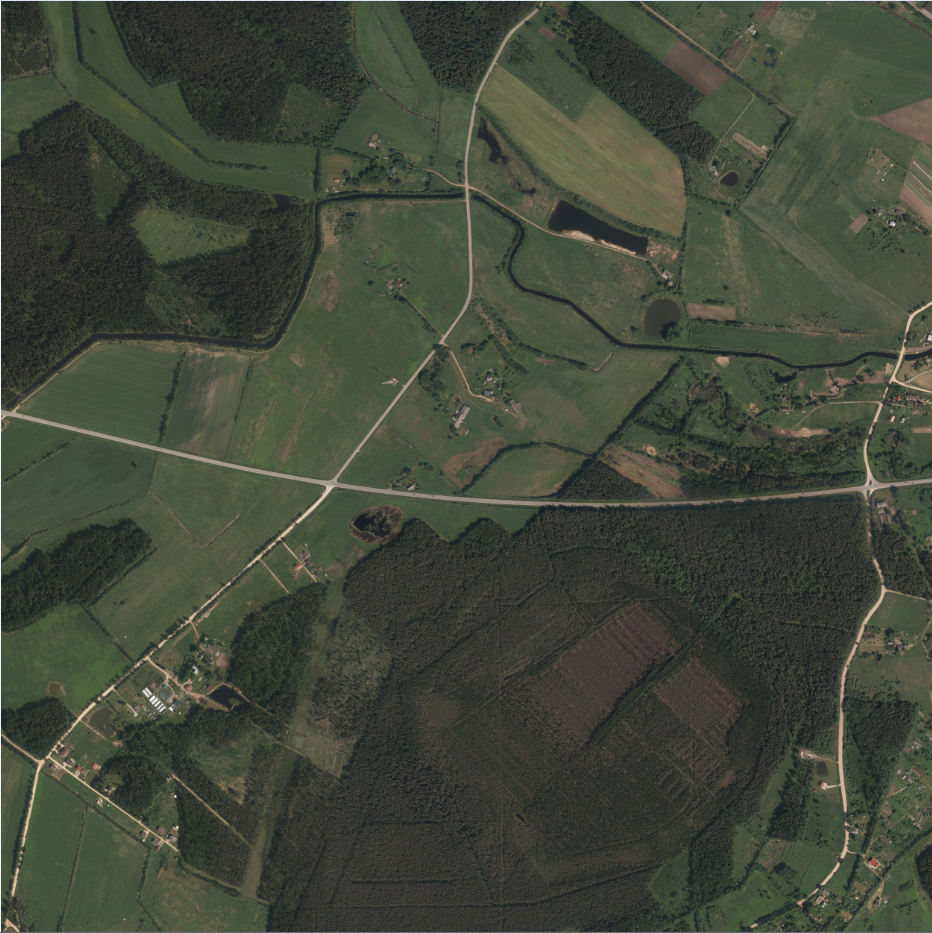
\includegraphics[width=0.6\textwidth]{original.png}
\caption{Maģistra darbā izmantotā ortofotokarte mērogā 1:10 000 © Latvijas Ģeotelpiskās informācijas aģentūra, 2013.}
\label{fig:fullIm}
\end{figure}\par
Maģistra darba īstenošanai, kā parauga dati tiek izmantoti tās pašas ortofotokartes fragmenti, kura tiek segmentēta un klasificēta zemes pārseguma tipos. 
\section{Pētāmais apgabals}
Pētāmais apgabals ir 16 $km^2$ plaša teritorija Ķekavas novadā, dienvidrietumu virzienā no Ķekavas un aptver Latvijai raksturīgu piepilsētas teritoriju. Pētāmais apgabals ir ļoti daudzveidīgs un ietver aramzemju platības, pļavas, kanālus, dīķus, viensētas, ciematu "Jaunsils", plašas mežu platības kā arī Augsto Tīreli pētāmā apgabala dienvidu un dienvidaustrumu daļā. Pētāmā apgabala atrašanās vieta redzama \ref{fig:lielaKarte} attēlā. \ref{fig:kekavaKarte} attēlā redzams kartes fragments, kas parāda, kādi vides objekti sastopami pētāmajā apgabalā.
\begin{figure}[h!]
\centering
\begin{subfigure}[b]{.49\linewidth}
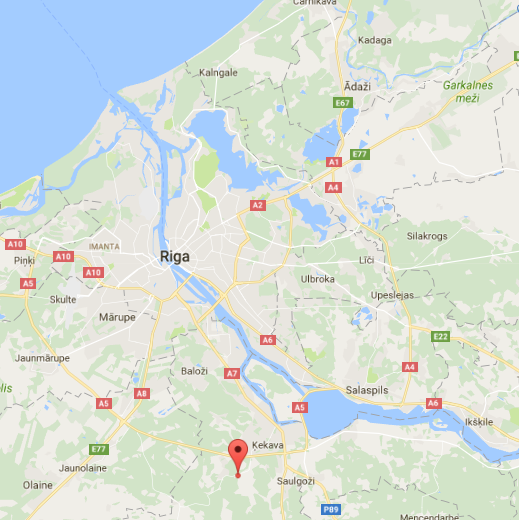
\includegraphics[width=\linewidth]{karte}
\caption{Pētāmā apgabala atrašanās vieta © Google, 2017.}\label{fig:lielaKarte}
\end{subfigure}
\begin{subfigure}[b]{.49\linewidth}
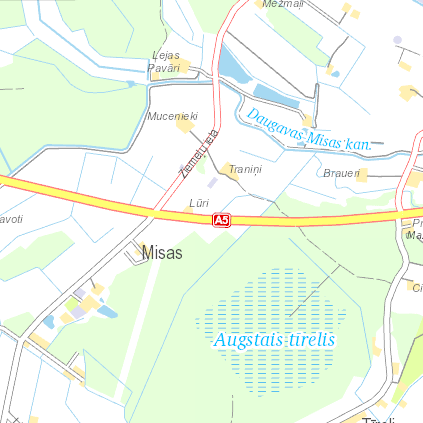
\includegraphics[width=\linewidth]{kekavaKarte}
\caption{Ķekavas apkārtnes karte © Valsts zemes dienests, pirmpublicējuma gads 1999-2012.}
\label{fig:kekavaKarte}
\end{subfigure}
\caption{Pētāmā apgabala ģeogrāfiskais novietojums.}
\end{figure}
\chapter{Zemes pārseguma atpazīšana augstas izšķirtspējas datos}
\section{Klasiskā pieeja: segmentācija un vadītā klasifikācija}
Klasiskā pieeja ortofotokartes sadalīšanai zemes pārseguma tipos sastāv no ortofotokartes segmentācijas un rezultātā iegūto segmentācijas reģionu klasifikācijas izmantojot kādu no mašīnmācīšanās metodēm. Šajā gadījumā segmentāciju veic, izmantojot krāsu attēlu segmentācijas metodi JSEG, bet rezultātus klasificē zemes pārseguma tipos, izmantojot vadītās klasifikācijas k-tuvāko kaimiņu metodi. Vadītā klasifikācija paredz, ka metode izmanto iepriekš sagatavotus parauga datus.
\subsection{Apmācības datu sagatavošana: deskriptoru rēķini}
\subsubsection{Deskriptori un tēli}Pēc tam, kad attēls ir sadalīts reģionos, nepieciešams izvēlēties un aprēķināt reģionu skaitliskās īpašības jeb deskriptorus, kas tiek izmantoti reģionu aprakstīšanai. To ir iespējams izdarīt, izmantojot reģiona ārējās raksturīgās īpašības, kā piemēram, reģiona robežu vai tā iekšējās īpašības, kā piemēram, pikseļu vērtību raksturlielumus, ko satur reģions. \cite{gonzalez2002digital}\par
Ārējos reģiona raksturlielumus izmanto, kad interesējošajam reģionam ir raksturīga specifiska forma, bet iekšējās raksturīgās īpašības izmanto, kad interesē reģiona krāsa un tekstūra. Reizēm nepieciešamā rezultāta sasniegšanai jāizmanto gan ārējās, gan iekšējās raksturīgās īpašības. Uzmanība jāpievērš tam, vai pazīmju vērtības (LZA, angl. \textit{feature}), kas tiek izvēlētas kā deskriptori (LZA, angl. \textit{descriptor}), būtiski neietekmē tādi pārveidojumi kā izmēra izmaiņas, rotācija un translācija.  \cite{gonzalez2002digital}\par
Tālāk apskatītas dažādas pieejas, kā raksturot attēla reģionu. Divi no reģiona vienkāršākajiem deskriptoriem ir tā platība (angl. \textit{area}), ko raksturo pikseļu skaits reģionā, un perimetrs jeb reģiona robežas garums pikseļos. Atsevišķi šos deskriptorus attēla reģiona raksturošanai izmanto tikai tādos gadījumos, ja reģiona izmēri un forma nemainās. Biežāk tiek izmantots tāds deskriptors, kā kompaktums (angl. \textit{compactness}). Kompaktumu izsaka, kā perimetra kvadrāta dalījumu ar platību ((perimetrs$^2)/$platība). Kompaktums ir bezdimensionāls lielums, kas ir mazs diska formas reģioniem. Citi vienkāršie deskriptori ir reģiona pelēko toņu vidējā (angl. \textit{mean}) vērtība un mediāna (angl. \textit{median}), reģiona maksimālā un minimālā pelēkā toņa vērtība, kā arī to pikseļu skaits, kas reģionā atrodami virs un zem reģiona vidējās vērtības. \cite{gonzalez2002digital}\par
Tēls ir deskriptoru vektors. Bieži tēlu pazīšanā tiek izmantots vārds "pazīme", ko attiecina uz deskriptoriem. Tēlu klase (LZA, angl. \textit{pattern class}) ir vairāku tēlu kopa, kam raksturīgas līdzīgas deskriptoru vērtības. Tēlu klases apzīmē ar $ \omega_1, \omega_2, ..., \omega_W $, kur $W$ apzīmē klašu skaitu. Automātiskā tēlu pazīšana sevī iekļauj tādas metodes, kur katrs tēls tiek piešķirts kādai klasei ar pēc iespējas mazāku iejaukšanos no cilvēka puses. Tēlu vektorus apzīmē ar treknrakstā izceltiem, mazajiem alfabēta burtiem un pieraksta formā 
\begin{equation}
\textbf{x}=\begin{bmatrix}
x_1\\ 
x_2\\ 
...\\ 
x_n
\end{bmatrix}
\end{equation}
kur katrs loceklis $ x_i $ apzīmē $i$-to deskriptoru un $n$ ir kopējais deskriptoru skaits. Tēla vektors ir attēlots kā kolonnas matrica ar izmēru $n \times 1$ un līdz ar to, to iespējams izteikt arī kā $ \textbf{x}=(x_1, x_2, ..., x_n)^T $, kur $^T$ apzīmē transponēšanas operāciju. \cite{gonzalez2002digital} \par
\subsubsection{Darbā izmantotie deskriptori}
Darbā kā deskriptori tiks izmantoti attēla reģiona vidējā vērtība, mediāna un standartnovirze. Katrs no šiem deskriptoriem arī turpinājumā tiek apskatīts detalizētāk.\par
Vidējā vērtība (LZA, angl. \textit{mean value}) attēlam ir aritmētiskā vidējā vērtība, un tā tiek definēta, kā visu spilgtuma vērtību summas dalījums ar apskatīto pikseļu skaitu. Attēla reģiona vidējā vērtība ir populārs raksturlielums. Vidējo vērtību $\mu _k$ atsevišķai krāsu joslai, kas sastāv no $n$ pikseļu vērtībām $BV_{i,k}$ aprēķina, izmantojot formulu:
\begin{equation}
\mu _k=\frac{\sum_{i=1}^{n}BV_{i,k}}{n}
\end{equation}
Lai attēlam aprēķinātu standartnovirzi (LZA, angl. \textit{standard deviation}), nepieciešams vispirms aprēķināt attēla dispersiju (LZA, angl. \textit{variance}). Attēla dispersija ir vidējā kvadrātiskā novirze visām pikseļu vērtībām no attēla vidējās vērtības. To aprēķina, izmantojot formulu:
\begin{equation}
var_k=\frac{\sum_{i=1}^{n}{(BV_{i,k}-\mu_k)^2}}{n}
\end{equation}
Attēla standartnovirze ir kvadrātsaknes vērtība no dispersijas un to aprēķina, izmantojot formulu:
\begin{equation}
s_k=\sqrt{var_k}
\end{equation}
Maza standartnovirze kādā attēla reģionā raksturo to, ka vērtības šajā reģionā ir tuvu reģiona vidējai vērtībai un vienas otrai. Turpretī, liela standartnovirzes vērtība nosaka to, ka pikseļu vērtības reģionā ir izkliedētas un atrodas tālu no vidējās vērtības. \cite{stdMeanMedian}\par
Attēla mediāna ir vērtība skaitļu virknē pēc pozīcijas, kad visas pikseļu vērtības ir sarindotas augošā secībā \cite{stdMeanMedian}.
\subsubsection{Praktiskā realizācija: datu sagatavošana un deskriptoru aprēķināšana}
\paragraph{Koordinātu pārrēķināšana reģionu failiem}
Lai veiktu deskriptoru aprēķinus iepriekš sagatavotajiem parauga datiem, parauga datu maskas nepieciešams sareizināt ar segmentācijas rezultātā iegūtajiem reģioniem. Lai izmantotu \textit{QGIS} spraudni deskriptoru rēķiniem, \textit{Matlab} vidē sagatavoto attēlu koordinātu sistēmai ir nepieciešams piesaistīt kartes projekcijas koordinātes. Šādu koordinātu pārrēķināšanu nepieciešams arī veikt segmentācijas rezultātā iegūtajam reģionu failam.\par 
Koordinātu sistēmu pārrēķina, izmantojot \textit{Python} skriptu. Skriptā vispirms importē bibliotēkas \textit{gdal} un \textit{osr}, kas nepieciešamas, lai veiktu koordinātu pārrēķināšanu, kā arī papildus funkcijas no faila \textit{additionalFunctions} (funkciju klase, kas ir izstrādāta VeA IZI “VSRC” projektu ietvaros), kurām turpmāk skriptā varēs piekļūt, izmantojot klases objektu \textit{af}. 
\begin{lstlisting}[language=Python]
import gdal
import osr
from additionalFunctions import additionalFunctions

af = additionalFunctions()
\end{lstlisting}\par
Pēc tam uzstāda mainīgā \textit{origPath} vērtību, norādot pilno ceļu, kur atrodama aerofotogrāfija, no kuras iespējams nolasīt ar kartes projekciju saistīto informāciju, \textit{imPath} ar pilno ceļu uz to direktoriju, kurā atrodami faili, kam nepieciešams mainīt koordinātu sistēmu (šajā gadījumā faili ar reģionu matricām) un \textit{names}, kas ir to failu nosaukumu masīvs, kam nepieciešams veikt koordinātu pārrēķināšanu.
\begin{lstlisting}[language=Python]
origPath = 'C:\Path\to\\aerophotography.tif'
imPath = 'C:\Path\to\region\folder\\'
names = ['citsRegion.tif', 'lauksRegion.tif', 'udensRegion.tif', 'zaliensRegion.tif', 'kokiRegion.tif', 'region.tif']
\end{lstlisting}\par
Tālāk, ciklā ejot cauri reģionu failiem, fails tiek atvērts un mainīgajā \textit{imb} tiek saglabāta attēla 1. rastra (LZA, angl. \textit{raster}) josla. Tad šī iegūtā rastra josla tiek ielasīta mainīgajā \textit{im} kā masīvs. Tālāk rīkojas ar oriģinālo aerofotogrāfiju to ielasot mainīgajā \textit{imd1} un iegūstot tās ar kartes projekciju saistīto informāciju, kas tiek saglabāta mainīgajā \textit{geot}.
\begin{lstlisting}[language=Python]
for n in names:
    imd = gdal.Open(imPath + n)
    imb = imd.GetRasterBand(1)
    im = imb.ReadAsArray()
    imd1 = gdal.Open(origPath)
    geot = imd1.GetGeoTransform()
\end{lstlisting}\par
Pēc tam, izmantojot \textit{osr} pakotnes klasi \textit{SpatialReference} tiek izveidots klases objekts ar nosaukumu \textit{Projection}, kas tiek aizpildīts, izmantojot projekcijas atsauci no oriģinālās aerofotogrāfijas. Tālāk, izmantojot iepriekš aizpildītās projekcijas, tiek iegūta informācija par EPSG ģeodēzisko parametru datu kopu. Izmantojot visu iepriekš iegūto informāciju tiek izveidots jauns fails, kas tiek saglabāts tajā pašā direktorijā, kur reģiona fails, kam bija nepieciešams mainīt koordinātas.
\begin{lstlisting}[language=Python]
	Projection = osr.SpatialReference()
    Projection.ImportFromWkt(imd1.GetProjectionRef())
    EPSG = (Projection.GetAttrValue("AUTHORITY", 1))
    rasterOrigin = [geot[0], geot[3]]
    af.array2raster(imPath + 'G' + n, rasterOrigin, geot[1], geot[5], im, 1, gdal.GDT_UInt16, 3059)
\end{lstlisting}\par
Lai veiktu projekciju pārrēķināšanu un veiksmīgi importētu nepieciešamās pakotnes, skriptu, izmantojot tā pilno ceļu, nepieciešams izpildīt no konsoles. Konsoli ar visām, vajadzīgajām importētajām bibliotēkām var atvērt izpildot \verb|C:\Program Files\QGIS 2.14\OSGeo4W.bat| failu.
\paragraph{Deskriptoru aprēķināšana, izmantojot \textit{QGIS} programmatūru}
Kad koordinātas pārrēķinātas visiem parauga datu reģionu failiem un segmentācijas rezultātā iegūtajam reģionu failam, tad iespējams aprēķināt deskriptorus, izmantojot programmatūru \textit{QGIS}. Darbā tiek izmantota \textit{QGIS 2.14.11-Essen} versija. Lai veiktu reģiona faila poligonizāciju, interesējošais fails tiek ielasīts \textit{QGIS} \textit{Browser Panel} logrīkā, veicot dubultklikšķi uz tā reģiona faila nosaukuma, ko nepieciešams ielasīt.\par
Attēla poligonizācija ir attēla sadalīšana dažādas formas un izmēru poligonos, veidojot poligonu tīklu. Katrā poligonā esošos pikseļus vieno kāda pazīme (šajā gadījumā reģiona numurs, kam pikseļi pieder). \cite{poly}\par
Tālāk \textit{Raster} $\rightarrow$ \textit{Conversion} $\rightarrow$ \textit{Polygonize} tiek atvērts poligonizācijas rīks, kur \textit{Input file} ir ielasītais reģionu fails, kam nepieciešams veikt poligonizāciju, bet pie \textit{Output file for polygons}, klikšķinot uz "Select" pogu atveras logs jaunas mapes izveidei, kur tiks uzglabāti poligonizācijas rezultāti. Kā redzams attēlā \ref{fig:poligonizacija}, pārējās opcijas un mainīgos atstājam nemainītus un, spiežot "OK", apstiprinām izvēli.
\begin{figure}[h!]
\centering
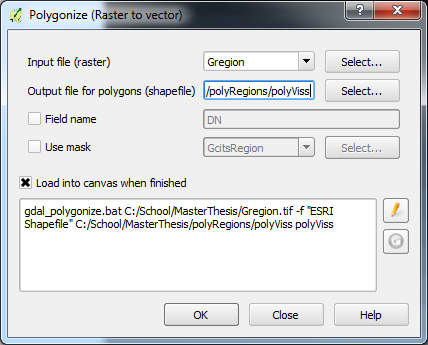
\includegraphics[scale=0.7]{polygonize} 
\caption{Rīks attēla poligonizācijai.}
\label{fig:poligonizacija}
\end{figure}\par
Iepriekš aprakstītās darbības tiek veiktas visiem reģionu failiem un gala rezultātā tiek iegūti 6 poligonu faili, kas redzami \ref{fig:poly} attēlā.
\begin{figure}[h!]
\centering
\begin{subfigure}[b]{.3\linewidth}
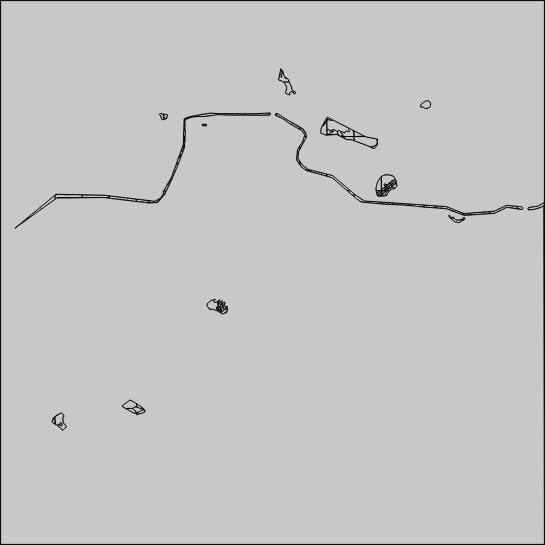
\includegraphics[width=\linewidth]{udensPolygons}
\caption{Poligonu attēls ūdens parauga datiem.}\label{fig:udensPoly}
\end{subfigure}
\begin{subfigure}[b]{.3\linewidth}
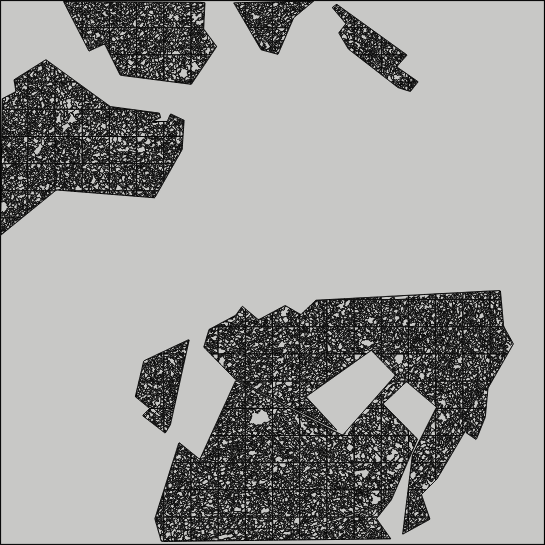
\includegraphics[width=\linewidth]{kokiPolygons}
\caption{Poligonu attēls koku parauga datiem.}
\label{fig:kokiPoly}
\end{subfigure}
\begin{subfigure}[b]{.3\linewidth}
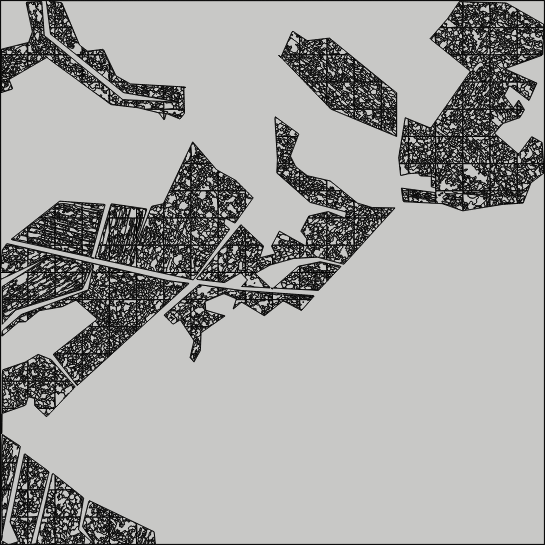
\includegraphics[width=\linewidth]{zaliensPolygons}
\caption{Poligonu attēls zāliena parauga datiem.}\label{fig:zaliensPoly}
\end{subfigure}
\begin{subfigure}[b]{.3\linewidth}
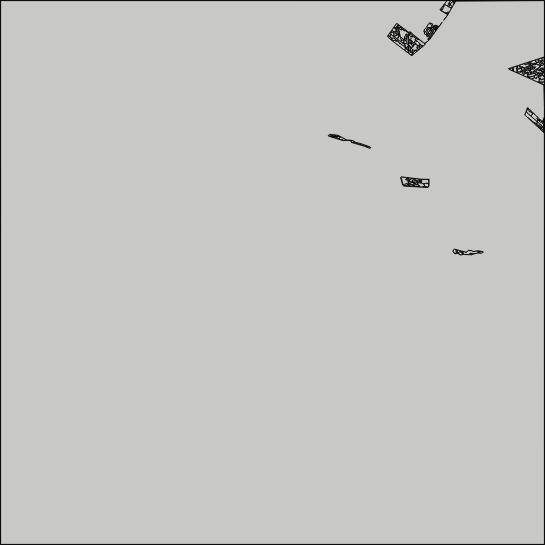
\includegraphics[width=\linewidth]{lauksPolygons}
\caption{Poligonu attēls lauku parauga datiem.}\label{fig:lauksPoly}
\end{subfigure}
\begin{subfigure}[b]{.3\linewidth}
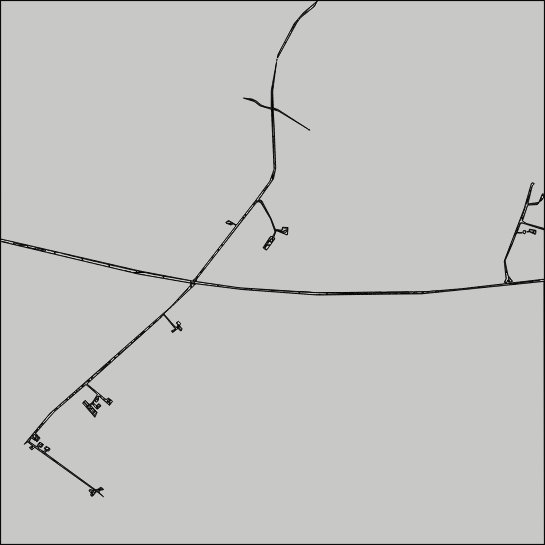
\includegraphics[width=\linewidth]{citsPolygons}
\caption{Poligonu attēls cita parauga datiem.}
\label{citsPoly}
\end{subfigure}
\begin{subfigure}[b]{.3\linewidth}
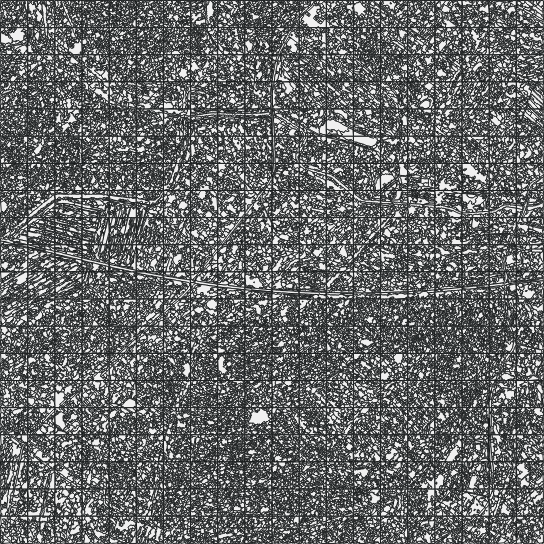
\includegraphics[width=\linewidth]{vissPolygons}
\caption{Poligonu attēls visiem reģioniem.}\label{vissPoly}
\end{subfigure}
\caption{Rezultāti pēc poligonizācijas.}
\label{fig:poly}
\end{figure}\par
Izmantojot \textit{Plugins} $\rightarrow$ \textit{Python Console}, augšējā joslā tiek nospiesta poga "Show Editor", lai atvērtu rīku \textit{Python} koda ievadīšanai. Šajā teksta logā ar pirmo komandu importējam pakotni \textit{QgsZonalStatistics}, kam pēc tam seko nodefinētas atrašanās vietas direktorijai ar poligonizācijas rezultātiem, poligonizācijas failu nosaukumiem un oriģinālajam attēlam, kā arī masīvs ar joslas apzīmējošiem burtiem. Tālāk ciklā katram poligonu failam ielasa tā poligonu slāni un ejot ciklā cauri katram attēla slānim aprēķina slānī esošo reģionu izmēru pikseļos, vidējo vērtību, mediānu un standartnovirzi.\par
Skripta augšpusē, nospiežot pogu "Run script", izpilda skriptu, kas pēc veiksmīgas skripta izpildes, deskriptorus saglabā atribūtu tabulā katram poligonu slānim.
\begin{lstlisting}[language=Python]
from qgis.analysis import QgsZonalStatistics

folder = 'C:/School/MasterThesis/polyRegions/'
pathes = ['polyCits/polyCits.shp', 'polyKoki/polyKoki.shp', 'polyLauks/polyLauks.shp', 'polyUdens/polyUdens.shp', 'polyZaliens/polyZaliens.shp',  'polyViss/polyViss.shp']
rasterFilePath = 'C:/School/3333-53_1.tif'
bands = ["R","G","B"]

for path in pathes:
    polygonLayer = QgsVectorLayer(folder+path, 'polygon', "ogr") 
    for i in range(1,4):
        zoneStat = QgsZonalStatistics (polygonLayer,  rasterFilePath, bands[i-1], i, QgsZonalStatistics.Count  | QgsZonalStatistics.Mean | QgsZonalStatistics.Median | QgsZonalStatistics.StDev)
        zoneStat.calculateStatistics(None)
\end{lstlisting}
Lai šos rezultātus saglabātu \textit{csv} failos, ar labo peles pogu uzspiežot uz interesējošā poligona faila, atver izvēlni, kur izvēlas opciju \textit{Save As...}, kas atver logrīku vektoru slāņa saglabāšanai. Iestatījumus atstāj gandrīz nemainītus, izņemot opciju faila nolasīšanai, kā redzams \ref{fig:csv} attēlā.
\begin{figure}[h!]
\centering
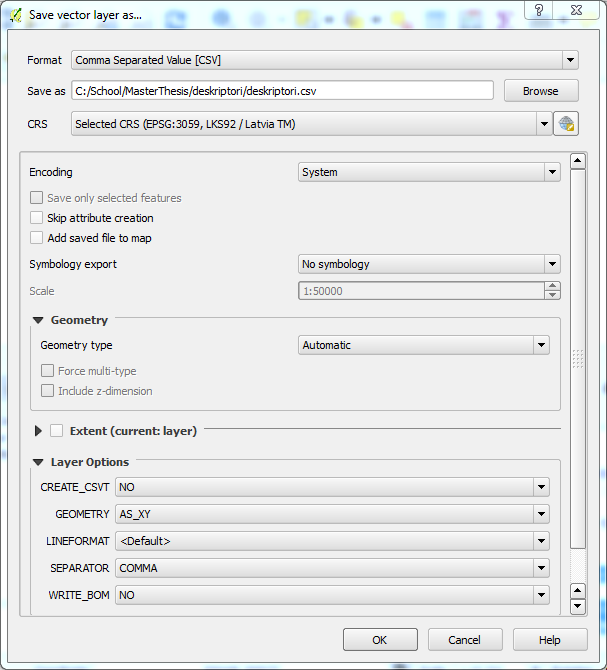
\includegraphics[scale=0.5]{saveAsCSV}
\caption{Logrīks deskriptoru saglabāšanai \textit{csv} formātā.}
\label{fig:csv}
\end{figure}\par
\paragraph{Deskriptoru matricu pēcapstrāde}Vispirms \textit{csv} failus atver kādā darba grāmatu apstrādes programmā un izdzēš kolonnas \textit{GCount} un \textit{BCount}. Pēc tam, kad \textit{MatLab} ielasīti \textit{csv} faili \textit{table} formātā, ielasītās deskriptoru tabulas pārvērš matricas formātā, izmantojot \textit{MatLab} iebūvēto funkciju \textit{table2array}. Pēc tam šo masīvu, kā parametru, padod funkcijai \textit{removeDublicates}, kas izdzēš tās rindiņas, kas manuālas datu atlases rezultātā veidojušas reģionu atgriezumus un, kuru deskriptori var būt sagrozītas vērtības mazo reģionu izmēru dēļ.\par 
Vispirms funkcija \textit{removeDublicates} atsevišķā matricā atlasa tikai tās rindiņas ar reģioniem, kur reģiona izmērs ir lielāks par 5 pikseļiem. Tad no šiem izmēra ziņā derīgajiem reģioniem nosaka unikālās reģionu identifikatoru vērtības. Ja iepriekš atlasītajā matricā, ciklā ejot cauri reģionu identifikatoriem, ir vairāk kā viena rindiņa ar vienu identifikatoru, tad šī reģiona identifikatoru pievieno matricai \textit{dublicateIds}.
\begin{lstlisting}
function result = removeDublicates(deskriptori)
	j=1;
	for i=1:length(deskriptori)
   		if(deskriptori(i,2)>5)
       		tempDeskriptori(j,:)=deskriptori(i,:);
       		j=j+1;
   		end
	end
	uniqueIds=unique(tempDeskriptori(:,1));
	j=1;
	for i=1:length(uniqueIds)
    	if sum(tempDeskriptori(:,1)==uniqueIds(i))>1
        	dublicateIds(j)=uniqueIds(i);
        	j=j+1;
    	end
	end
\end{lstlisting}
Pēc tam ciklā, ejot cauri to reģionu identifikatoriem, kas masīvā atkārtojas, atlasa tās rindiņas, kam ir viens reģiona identifikators un izveido pagaidu masīvu, kur uzglabā šo atkārtojošo rindiņu reģionu identifikatorus un izmērus. No tikko aizpildītā pagaidu masīva atrod to reģiona daļu, kam ir vislielākais izmērs un tā rindiņu ar visiem deskriptoriem ievieto gala rezultāta masīvā. Pašās funkcijas beigās no gala rezultāta masīva izdzēš kolonnu ar reģionu izmēriem.
\begin{lstlisting}
	k=1;
	for i=1:length(dublicateIds)
    	dublicateRows=find(tempDeskriptori(:,1)==dublicateIds(i));
    	temp=zeros(length(dublicateRows),2);
    	for j=1:length(dublicateRows)
        	temp(j,1)=dublicateRows(j);
        	temp(j,2)=tempDeskriptori(dublicateRows(j),2);
    	end
    	maxCount=max(temp(:,2));
    	for j=1:length(dublicateRows)
        	if temp(j,2)==maxCount
            	result(k,:)=tempDeskriptori(dublicateRows(j),:);
            	k=k+1;
        	end
    	end
	end
	result(:,2)=[];
\end{lstlisting}\par
Iepriekš aprakstītās darbības izpilda visiem \textit{csv} failiem, kas satur sevī deskriptorus parauga datiem un visiem reģioniem. Kad iegūtas visas tabulas bez dublikātu rindiņām vienam un tam pašam reģionam, parauga datu deskriptoru matricas apvieno, izmantojot \textit{MatLab} iebūvēto funkciju \textit{vertcat}, ievērojot secību. Secība ir būtiska, jo nepieciešams izveidot kolonnas vektoru ar klašu atzīmēm parauga datiem. Klašu atzīmes ir skaitļi, kas nosaka kāds skaitlis atbilst katrai klasei. Pēc tam, kad klašu atzīmju vektors ir izveidots, var veikt pēdējās darbības gan parauga datu deskriptoriem, gan visu reģionu deskriptoru matricām - atbrīvoties no reģionu identifikatoru kolonnas un normalizēt deskriptorus, izmantojot \textit{MatLab} iebūvēto funkciju \textit{zscore}.
\begin{lstlisting}
sampleDescr=vertcat(udensDescr, kokiDescr, zaliensDescr, lauksDescr, citsDescr);

a=length(udensDescr);
b=a+length(kokiDescr);
c=b+length(zaliensDescr);
d=c+length(lauksDescr);

class_labels=1:5;
sampleClasses(1:a)=class_labels(1);
sampleClasses(a+1:b)=class_labels(2);
sampleClasses(b+1:c)=class_labels(3);
sampleClasses(c+1:d)=class_labels(4);
sampleClasses(d+1:length(sampleDescr))=class_labels(5);
sampleClasses=sampleClasses';

sampleDescr(:,1)=[];
vissDescr(:,1)=[];

sampleDescr=zscore(sampleDescr);
vissDescr=zscore(vissDescr);
\end{lstlisting}
\subsection{JSEG un tā realizācija}
\subsubsection{JSEG metodes teorētiskais apskats}JSEG jeb J-segmentācija ir krāsu attēlu segmentācijas algoritms, kas reģionu atrašanas procesā izmanto gan krāsas, gan tekstūras informāciju \cite{1colImSegm1999}. Attēlu segmentācija datorredzē ir digitālā attēla sadalīšanas process vairākos segmentos jeb pikseļu kopās, savienojot kaimiņpikseļus ar līdzīgām raksturīpašībām. Segmentācijas mērķis ir vienkāršot vai mainīt attēla reprezentāciju formā, kas ir daudz nozīmīgāka un vieglāk analizējama. \cite{shapiro2001computer}, \cite{cleve2008classification}\par
Pats algoritms sastāv no pieciem soļiem, kur katrs no tiem tiks detalizēti aprakstīts tālākajos punktos.
\paragraph{Krāsu attēlu kvantizācija}Lai atšķirtu līdzīgos krāsu reģionus no citiem, vispirms attēlu nepieciešams kvantizēt jeb samazināt tajā esošo krāsu skaitu. Krāsu attēlu kvantizācija ir process, kurā tiek samazināts atšķirīgo toņu skaits attēlā, ar mērķi, lai jaunais attēls būtu maksimāli līdzīgs iepriekšējam attēlam. Šādā veidā netiek būtiski ietekmēta attēla vizuālā kvalitāte, kā arī netiek zaudēta vērtīgā informācija, bet attēls tiek pārveidots tādā formā, ka to reprezentē tikai pāris krāsu. Krāsu attēliem, kas satur dabas ainavas, parasti izvēlas 10-20 krāsas, kas salīdzinoši efektīvi spēj reprezentēt attēlā redzamo krāsu gammu.\cite{1colImSegm1999}\par
Pēc krāsu kvantizācijas katram attēla pikselim tiek piešķirts kvantizācijas rezultātā atrastās krāsas numurs. Krāsu klase ir visu to pikseļu kopa, kam piešķirta konkrētā kvantizētā krāsa. Pēc tam tiek izveidota krāsu tabula (LZA, angl. \textit{color map}), kur katrs attēla pikselis tam atbilstošajās koordinātās $(x,y)$ krāsu tabulā tiek aizstāts ar atzīmi, kurai krāsu klasei tas pieder.\cite{1colImSegm1999}\par
Pareiza krāsu kvantizācija ir ļoti nozīmīga segmentācijas sastāvdaļa, kas var ietekmēt galarezultātu.
\paragraph{Labi segmentēta attēla nosacījums}Tiek ieviesta vērtība J, kuru definē tālāk apskatītās formulas. Vispirms pieņemam, ka $Z$ ir $N$ punktu kopa no krāsu kartes, kas sastāv no punktiem $z=(x,y)$, \(z \in Z\) un, ko raksturo vidējā vērtība $m$, 
\begin{equation}
m=\frac{1}{N}\sum_{z \in Z}z
\end{equation}
Pieņem, ka $Z$ sastāv no $C$ klasēm $Z_i, i=1,...,C$. Tādā gadījumā $m_i$ ir $N_i$ punktu vidējā vērtība klasē $Z_i$, 
\begin{equation}
m_i=\frac{1}{N_i}\sum_{z \in Z_i}z
\end{equation}
Ja
\begin{equation}
S_T=\sum_{z \in Z}\left \| z-m \right \|^2
\end{equation}
un
\begin{equation}
S_W=\sum_{i=1}^{C}S_i=\sum_{i=1}^{C} \sum_{z \in Z_i} \left \| z-m_i \right \|^2
\end{equation}
tad J definē kā
\begin{equation}
J=\frac{S_B}{S_W}=\frac{(S_T-S_W)}{S_W}
\end{equation}
Šis mērs nosaka, cik labi atšķirami ir dažādi krāsu klašu reģioni attēlā - jo lielāka J vērtība, jo tā krāsu klases ir labāk atšķiramas, homogēnas un krāsu klasei piederīgie pikseļi tuvāki viens otram vērtību ziņā.\cite{1colImSegm1999}\par
Lai noteiktu, kāds ir labs segmentācijas rezultāts, ieviešam mainīgo $\bar{J}$, kas tiek aprēķināts kā vidējā vērtība visiem segmentētajiem reģioniem tā vietā, lai to aprēķinātu uzreiz visam attēlam. Šāda mainīgā vērtību aprēķina
\begin{equation}
\bar{J}=\frac{1}{N}\sum_k M_k J_k,
\end{equation}
kur $J_k$ ir reģiona $k$ $J$ vērtība, $M_k$ punktu skaits reģionā $k$ un $N$ kopējais punktu skaits klašu kartē, bet summēšana notiek pa visiem reģioniem $k$. Šādi ieviests mainīgais ievieš jaunu kritēriju segmentācijas kvalitātes noteikšanai, kur labāko segmentācijas kvalitāti izsaka mazākā iespējamā $\bar{J}$ vērtība pār visiem reģioniem $k$. \cite{1colImSegm1999}\par
\paragraph{J-attēla izveide}Tomēr iepriekš aprakstītā kritērija pielietošana nav praktiska. Tādēļ tiek ieviests tāds jēdziens, kā J-attēls. J-attēls ir melnbalts attēls, kura pikseļu vērtības veido $J$ vērtība, kas aprēķināta interesējošā pikseļa apkārtnē ar izvēlētu rādiusu. Šādam attēlam raksturīga kalniem un ielejām līdzīga struktūra, kur tumšākās vērtības norāda tos pikseļus, kas vairāk koncentrēti kāda krāsu reģiona centrā, bet gaišākās vērtības pretēji attiecināmas uz krāsu reģiona robežu.\cite{2unsupImSegm2001}\par
Interesējošā pikseļa apkārtnes izmērs tiek izvēlēts balstoties uz nepieciešamo atšķiramo reģionu izmēriem, kā arī reģionu robežas detaļu smalkuma. Attiecīgi izmantojot mazāku loga izmēru iespējams izšķirt smalkākas detaļas un reģionus, kurus sastāda atsevišķas detaļas, bet liels loga izmērs ir izdevīgs tajos gadījumos, kad nepieciešams izšķirt reģionus, ko raksturo specifiska tekstūra. \cite{1colImSegm1999}\par
Lai noteiktu kāda pikseļa piederību konkrētajam reģionam, bet, lai nerastos novirzes taisnstūra formai līdzīgu reģionu dēļ, loga forma ir izvēlēta līdzīga aplim vai kvadrātam ar noapaļotiem stūriem. Apļi ir pieejami dažādos mērogos, kur katrs nākamais ir ar divas reizes lielāku rādiusu kā iepriekšējais. \cite{1colImSegm1999}\par
\paragraph{Reģionu audzēšana}J-attēla raksturīgās īpašības ļauj izmantot reģionu audzēšanas algoritmus attēla segmentācijā. Ja pieņem, ka sākumā viss attēls uzskatāms par veselu reģionu, tad kā redzams tabulā \ref{tab:logiUnMerogi}, algoritms jāsāk tādā mērogā, kāds ir nosakāms pēc reģiona izmēra. Piemēram, gadījumā, ja attēls nepārsniedz 512 pikseļus platumā un/vai garumā, bet ir lielāks par 256 pikseļiem, algoritms jāsāk no 3. mēroga soļa. \cite{2unsupImSegm2001}\par
\begin{table}[!ht]
\centering
\caption{Logu izmēri pie dažādiem mērogiem.}
\label{tab:logiUnMerogi}
\begin{tabular}{|p{1.5cm}|p{3.8cm}|p{3.8cm}|p{3.8cm}|}
\hline
Mērogs&Loga izmērs (pikseļos)&Reģiona izmērs (pikseļos)&Min. ielejas izmērs (pikseļos)\\ \hline \hline
1&9 x 9&64 x 64&32 \\ \hline
2&17 x 17&128 x 128&128 \\ \hline
3&33 x 33&256 x 256&512 \\ \hline
4&65 x 65&512 x 512&2048 \\ \hline
\end{tabular}
\end{table}
Pirmais solis ir noteikt, kuri pikseļi veidos tā saucamo ielejas sēklas pikseļu kopu. Viens variants ir aprēķināt katra reģiona vidējo vērtību un standartnovirzi, apzīmējot tās ar $\mu_J$ un $\sigma_J$ un ieviest sliekšņa vērtību $T_J$. 
\begin{equation}
T_j=\mu_J+a \sigma_J
\end{equation}
Šajā gadījumā $a$ ir kāda vērtība no skaitļu masīva $[-0.6, -0.4, -0.2, 0, 0.2, 0.4]$. Tas, kura vērtība no masīva tiek izmantota, tiek noteikts eksperimentālā veidā, balstoties uz to, kura vērtība garantē vislielāko ielejas punktu skaitu. Iepriekš ieviestā sliekšņa vērtība tiek pielāgota visām lokālajām $J$ vērtībām un tās, kuras ir mazākas par šo vērtību, tiek sauktas par ielejas punktu kandidātiem. Ielejas kandidātu punktus savieno izmantojot 4-savienojamību un tā tiek iegūti ieleju kandidāti. Ja šādas ielejas izmērs ir lielāks nekā norādīts \ref{tab:logiUnMerogi} tabulā, tad tādu kandidātu nosaka par ieleju. \cite{1colImSegm1999}\par
Tā kā audzēt reģionu pikseli pa pikselim ir ļoti lēni, tiek izmantota citādāka pieeja. Vispirms ielejās aizpilda caurumus un atrod tās $J$ vērtības, kuras ir zemākas par visu nesegmentēto pikseļu vidējo $J$ vērtību. $J$ vērtības, kas ir zemākas par vidējām vērtībām, savā starpā savieno un, ja tās atrodas blakus vienai vienīgai ielejai, tad pievieno tai. Tālāk pārvietojas uz nākamo mazāko mērogu un atkal atkārto iepriekš aprakstītās darbības ar to $J$ vērtību atrašanu, kuru vērtība mazāka nu jau par nākamā mēroga vidējo $J$ vērtību un to pievienošanu ielejai. Šādi turpina līdz sasniegts mazākais mērogs, kad pikseļu pievienošana jau notiek pa vienam. Pievienošanu sāk ar to, kam mazākā $J$ vērtība, un tajā brīdī nepievienotie pikseļi tiek uzglabāti buferatmiņā (LZIA, angl. \textit{buffer}) katru reizi informāciju par nepievienotajiem pikseļiem atjaunojot. \cite{1colImSegm1999}\par
\paragraph{Reģionu apvienošana}Standarta JSEG algoritmā reģionu apvienošana tiek veikta kā pēdējais solis. Reģionus apvieno izmantojot to, ka kvantizēto krāsu attēlā katram reģionam iespējams izveidot histogrammu, uz kuru balstoties tiek noteikta reģionu līdzība. Vispirms tabulā tiek aprēķinātas katru 2 blakus esošo kaimiņreģionu krāsu distances un tad šie reģioni, ar mazāko krāsas distanci starp pārējām, tiek apvienoti. Apvienotajam reģionam atkal tiek aprēķināta krāsas distance ar kaimiņreģioniem un informācija par distancēm tabulā tiek atjaunota. Process tiek atkārtots līdz tiek sasniegta iepriekš noteikta maksimāla sliekšņa vērtība. Iegūtais rezultāts arī ir attēla segmentācijas galarezultāts.\cite{1colImSegm1999}\par 
Literatūras avotā \cite{3seededRegGrow2005}, kā viens no JSEG metodes trūkumiem, tiek minēts tā segmentācijas rezultātu izteiktā sadrumstalotība salīdzinoši ar automātisko reģionu audzēšanas algoritmu no sēklas pikseļiem. To iespējams labot pēc segmentēšanas iegūtos reģionus klasificējot, izmantojot labu klasifikācijas algoritmu. Kā minēts pētījumos \cite{1colImSegm1999}, \cite{2unsupImSegm2001}, \cite{6buildings2008} un \cite{5forest2007} JSEG metodes priekšrocības, salīdzinoši ar citām attēlu segmentācijas metodēm, ir:
\begin{itemize}
\item Nav nepieciešams tekstūras modeļa parametru novērtējums;
\item Algoritms ir piemērots automātiskai attēlu apstrādei;
\item Algoritms necieš no trokšņa izraisītiem traucējumiem.
\end{itemize}
\subsubsection{JSEG metodes realizācija krāsu attēlu segmentācijā}Tālāk apskatīsim JSEG implementāciju aerofotogrāfijas segmentācijai. Autore eksistējošu JSEG implementāciju programmatūrā \textit{MatLab} optimizēja un pielāgoja pētījuma vajadzībām. Algoritmu iespējams izpildīt jebkurai aerofotogrāfijai, kas saglabāta TIFF formātā jeb tas ir 3 dimensiju attēls , kura vērtības ir 8 bitu veseli skaitļi bez zīmes (LZA, angl. \textit{unsigned integer}) (uint8). \par
Kā pats pirmais solis metodes implementācijā ir aerofotogrāfijas ielasīšana, kas tiks saglabāta 3 dimensiju matricā \textit{f}. Tālāk šī matrica \textit{f} tiek padota kā viens no parametriem metodei \textit{mainJSEG}. Metode \textit{mainJSEG} kā ievadparametrus saņem veselu skaitli (\textit{parts}), 3 dimensiju matricu \textit{f}, ko jau iepriekš apskatījām un veselu skaitli \textit{kmeansK}. Parametrs \textit{parts} raksturo to, cik daļās tiks sadalīts attēls gan horizontāli, gan vertikāli, bet \textit{kmeansK} nosaka kvantizācijai izmantotā pudurošanas pēc vidējiem (LZA, angl. \textit{k-means clustering}) \textit{k} parametru. Šī metode izvada reģionu matricu \textit{regions} un kvantizēto attēlu \textit{ImgQ}. Tālāk detalizētāk apskatīsim pašu \textit{mainJSEG} funkciju. \par
Vispirms izveidojam tukšu divdimensiju \textit{region} matricu tādā pašā izmērā, kā aerofotogrāfija, aprēķinam aerofotogrāfijas daļas izmēru, cik lielai daļai tiks veikti aprēķini vienā cikla reizē un izveidojam direktoriju starprezultātu uzglabāšanai. JSEG segmentācija tiek veikta ejot cauri kā horizontāli, tā vertikāli visiem aerofotogrāfijas apakšapgabaliem un vispirms aprēķinot katra apakšapgabala koordinātas, jo pēdējiem apakšapgabaliem kā rindā, tā kolonnā, var nebūt standarta izmērs (vienāds ar pārējiem ar apakšapgabaliem). Tālākajā koda fragmentā redzams, kā tiek izvēlēts apakšapgabals $[i,j]$ un izmantojot pudurošanu pēc vidējiem, tam tiek veikta kvantizācija, kuras rezultāts tiek atgriezts kā karte (matrica \textit{map}) ar tādu pašu izmēru, kā apakšapgabalam.
\begin{lstlisting}
subIm=image(((i-1)*partSize)+1:endOfImV,((j-1)*partSize)+1:endOfImH,:);
%------------K-means--------------------------------------------------%
[m,n,d] = size(subIm);
subIm=im2double(subIm);
X = reshape(subIm, m*n,d);
clusters = kmeans(X,kmeansK);
map = reshape(clusters, m, n);
\end{lstlisting}\par 
\begin{figure}[h!]
\centering
\begin{subfigure}[b]{.4\linewidth}
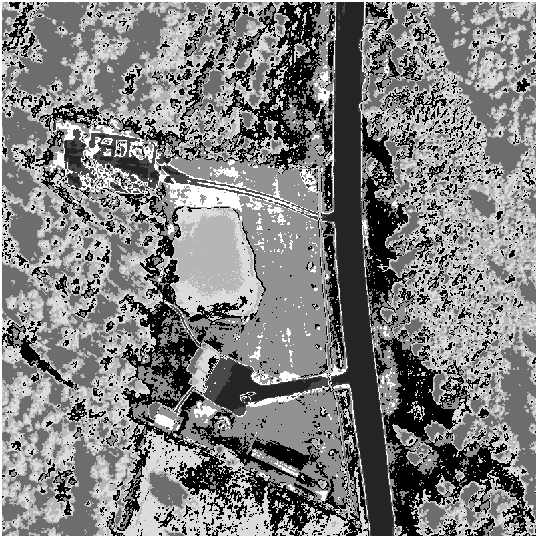
\includegraphics[width=\linewidth]{map8part}
\caption{Klašu karte.}
\label{kmeans8map}
\end{subfigure}
\begin{subfigure}[b]{.4\linewidth}
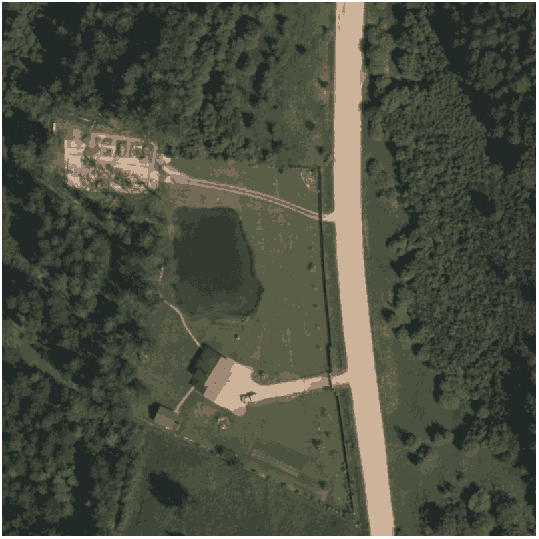
\includegraphics[width=\linewidth]{ImgQ8part}
\caption{Kvantizēts ortofotokartes fragments.}
\label{kmeans8imgq}
\end{subfigure}
\caption{Pudurošanas pēc vidējiem gala rezultāts ortofotokartes fragmentam, ja $k=8$.}
\label{fig:kmeans8}
\end{figure}
Pudurošanas pēc vidējiem parametrs \textit{k} ir viens no nozīmīgākajiem parametriem JSEG segmentācijā, kas nosaka to, cik daudz daļās tiks segmentēts attēls. \ref{fig:kmeans8} attēlā redzama klašu karte, ja pudurošanas pēc vidējiem parametrs $k=8$ un klašu kartei atbilstošais kvantizētais attēls.
\begin{figure}[h!]
\centering
\begin{subfigure}[b]{.4\linewidth}
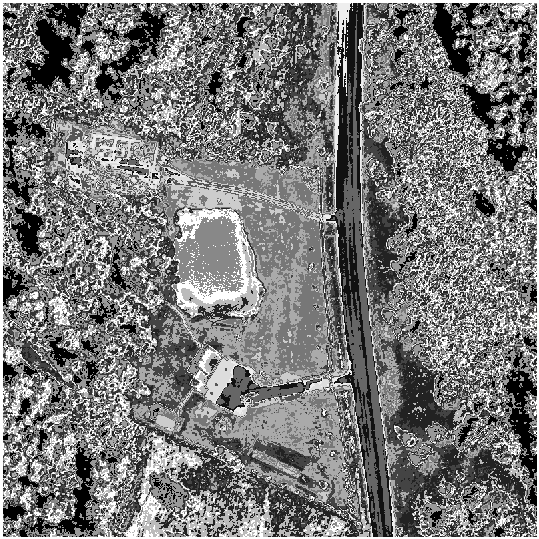
\includegraphics[width=\linewidth]{map16part}
\caption{Klašu karte.}
\label{kmeans16map}
\end{subfigure}
\begin{subfigure}[b]{.4\linewidth}
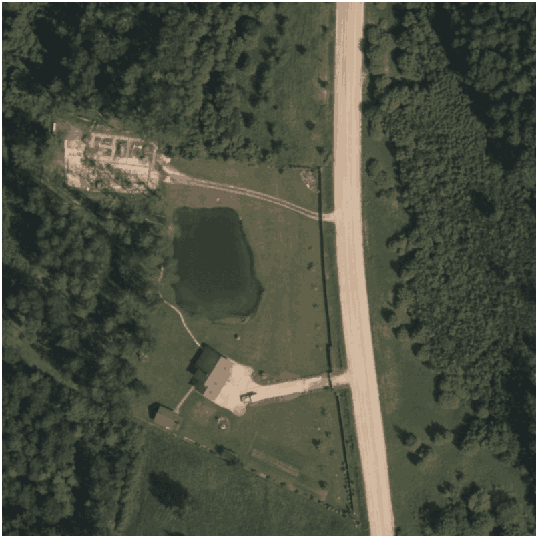
\includegraphics[width=\linewidth]{ImgQ16part}
\caption{Kvantizēts ortofotokartes fragments.}
\label{kmeans16imgq}
\end{subfigure}
\caption{Pudurošanas pēc vidējiem gala rezultāts ortofotokartes fragmentam, ja $k=16$.}
\label{fig:kmeans16}
\end{figure}
Toties \ref{fig:kmeans16} attēlā redzama klašu karte un tai atbilstošais kvantizētais ortofotokartes fragments, ja pudurošanas pēc vidējiem parametrs $k=16$. Salīdzinot \ref{fig:kmeans8} un \ref{fig:kmeans16} attēlus, redzams, ka visizteiktāk krāsu samazināšana ietekmējusi ūdens platības, zālāju un ceļu, kam raksturīga viendabīga tekstūra, bet vismazāk ietekmējusi koku vainagu pārsegumu. Protams, pudurošanas pēc vidējiem parametrs \textit{k} ir jāpielāgo arī apskatāmā attēla izmēram un dabas daudzveidībai tajā. Maza parametra vērtība var sniegt labus rezultātus mazā attēlā, bet lielākos attēlos vai tādos, kuros sastopama plaša dabas daudzveidība, var tikt nevajadzīgi sapludināti dažādi zemes pārseguma tipi.\par
Tālāk izmantojot jau klašu karti, tiek veikta J-attēla izveide. J-attēla izveide tiek veikta četros mērogos, kas gala rezultātā veido četrus J-attēlus - \textit{JI1, JI2, JI3, JI4}, kur \textit{JI1} vissmalkākais, bet \textit{JI4} attiecīgi izmantojot vislielāko mērogu. Tā kā visos mērogos J-attēla izveide ir vienāda, apskatīsim sīkāk tikai J-attēla izveidi smalkākajā mērogā ar loga izmēru 9. Šajā gadījumā funkcijai \textit{JImage} tiek padota klašu karte \textit{map} (funkcijā parametrs \textit{I}), loga izmērs (funkcijā parametrs \textit{ws}), kas, kā jau minēts, vienāds ar 9 un minimālā loga izmērs (funkcijā parametrs \textit{minWindow}), kas šajā gadījumā sakrīt ar loga izmēru. Izvadparametrs ir J-attēla matrica \textit{JI1}. \par
Funkciju sākam ar klašu kartes izmēru \textit{m} un \textit{n} iegūšanu, kā arī aprēķinam parametru \textit{d}, kas noteiks, ik pa cik pikseļiem, tiks veidots attēls J-attēla izveidošanai un loga diametru \textit{wswidth}. Līdzīgi, kā \textit{mainJSEG} funkcijā, izveidojam tukšu matricu \textit{JI}. Tālāk katram punktam $[i,j]$ no klašu kartes \textit{I} tiek aprēķināta tā apkārtnes robežu punkti un izmēri. Gadījumā, ja robežu vērtības pārsniedz klašu kartes izmērus vai tās ir negatīvas, tās tiek aizstātas ar minimālajām vai maksimālajām iespējamām vērtībām. 
\begin{lstlisting}
x1 = i-wswidth;
x2 = i+wswidth;
y1 = j-wswidth;
y2 = j+wswidth;
if x1<1; x1 = 1; end
if x2>m; x2 = m; end
if y1<1; y1 = 1; end
if y2>n; y2 = n; end
wid = x2-x1+1;
hei = y2-y1+1;
\end{lstlisting}
Pēc tam tiek aprēķināta standartnovirze izmantojot aprēķinātos loga izmērus un atrašanās vietu un šī standartnovirze tiek izmantota, kā viens no parametriem J vērtības aprēķināšanai funkcijā \textit{JCalculation}, kas bez standartnovirzes vēl kā ievadparametru saņem katru \textit{d}-to pikseli no klašu kartes \textit{I} diapozonā no \textit{x1} līdz \textit{x2} un no \textit{y1} līdz \textit{y2}. Sīkāk šīs funkcijas aprakstīšanā neiedziļināsimies, tikai ir vērts piebilst, ka šī funkcija atgriež J vērtību punktam $[i,j]$, kas arī tiek saglabāta iepriekš sagatavotajā, tukšajā matricā \textit{JI}. Ar to arī \textit{JImage} funkcijas apskatu var pabeigt.
\begin{lstlisting}
if wid == ws && hei == ws
	St = 1080; 
else
	wid=length(1:d:wid);
    hei=length(1:d:hei);
    reg=ones(wid,hei);
    M = [mean(1:wid), mean(1:hei)];
    [z1, z2] = find(reg);
    z = [z1, z2];
    St = sum(sqdist(z', M'));
end
JI(i,j) = JCalculation(I(x1:d:x2, y1:d:y2), St);
\end{lstlisting}\par
Atgriežoties pie \textit{mainJSEG} apskata, nākamais solis ir cilvēka acij patīkama kvantizētā attēla sagatavošana apakšapgabalam \textit{subIm}. Lai to izdarītu, funkcijai \textit{class2Img} tiek padota attiecīgā apakšapgabala klašu karte \textit{map} (funkcijā \textit{class_map}) un paša apakšapgabala matrica \textit{subIm} (funkcijā \textit{OrI}). Kā izvadparametrs, tiek veidota matrica \textit{partImgQ} (funkcijā \textit{Img}). Kā jau pārējās funkcijās, arī šajā vispirms tiek noteikti apakšapgabala izmēri (\textit{m, n, d}) un izveidota tāda paša izmēra matrica \textit{partImgQ} (\textit{Img}) uzglabāšanai. Tālākajā koda fragmentā katrai klasei no klašu kartes tiek atbilstoši pa attēla slāņiem aprēķināta vidējā vērtība un visu klasei piederošo pikseļu vērtības tiek ar to aizstātas.
\begin{lstlisting}
for i = 1:max(class_map(:))
	sq = find(class_map == i);
	for j = 1:d       
	    Channel = OrI(:,:, j);
	    u = mean(Channel(sq));
	    Channel = zeros(m,n);
	    Channel(sq) = u;
		Img(:,:, j) = Img(:,:,j) + Channel;
	end
end
\end{lstlisting} \par
Pēc cilvēka acij tīkama, kvantizēta attēla iegūšanas nepieciešams veikt ieleju identifikāciju. Ieleju identifikāciju veic funkcija \textit{ValleyD}. Funkcijai, kā parametri, tiek padota J-attēla matrica \textit{JI4} (funkcijā parametrs \textit{JI}) vislielākajā mērogā, pats mērogs (funkcijā parametrs \textit{scale}), kas šajā gadījumā ir 4, J-attēla vidējā vērtība \textit{uj} un standartnovirze \textit{sj}. Vispirms tiek atrasti matricas izmēri \textit{m, n} un \textit{d} un izveidota tukša matrica \textit{ValleyI} rezultāta uzglabāšanai. Tad tiek ieviests specifisks masīvs \textit{a}, kas satur $[-0.6, -0.4, -0.2, 0, 0.2, 0.4]$, noteikts minimālais ielejas izmērs \textit{scale}, balstoties uz mērogu, un pagaidām atrastais maksimālais ielejas izmērs uzstādīts vienāds ar nulli. Zemāk esošajā koda fragmentā, izmantojot katru masīva \textit{a} elementu, tiek aprēķina sliekšņa vērtība \textit{TJ}, kuru izmantojot tiek atrasti kandidātu ieleju punkti \textit{VP}. Izmantojot 4-savienojamību un minimālā ielejas izmēra vērtību \textit{scale}, tiek atrastas ielejas. Ja šo atrasto ieleju izmērs pie konkrētās \textit{a} vērtības lielāks, kā atrastais maksimālais ielejas izmērs, tad tās tiek saglabātas izvadparametrā \textit{ValleyI} un tagadējais maksimālās ielejas izmērs \textit{MaxVSize} tiek atjaunots.
\begin{lstlisting}
for i = 1:length(a)
	TJ = uj + a(i)*sj;
	VP = false(m,n);
	VP(JI <= TJ) = 1;
	VP_lab = bwlabel(VP,4);
	VPlab_hist = histc(VP_lab(:),1:max(VP_lab(:)));
	sq = find(VPlab_hist>=scale);
	VSize = length(sq);
	if length(sq)>MaxVSize
		ValleyI = zeros(m, n);
		for  k = 1:length(sq)
			ValleyI(VP_lab==sq(k))=k;
		end
		MaxVSize = VSize;
	end   
end
\end{lstlisting}\par
\begin{figure}[h!]
\centering
\begin{subfigure}[b]{.3\linewidth}
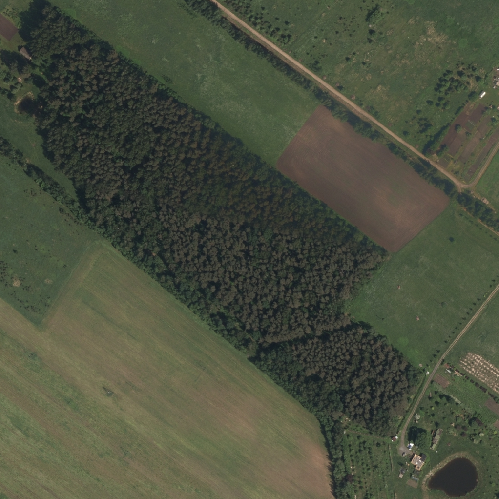
\includegraphics[width=\linewidth]{testImagepart}
\caption{RGB attēls.}
\end{subfigure}
\begin{subfigure}[b]{.3\linewidth}
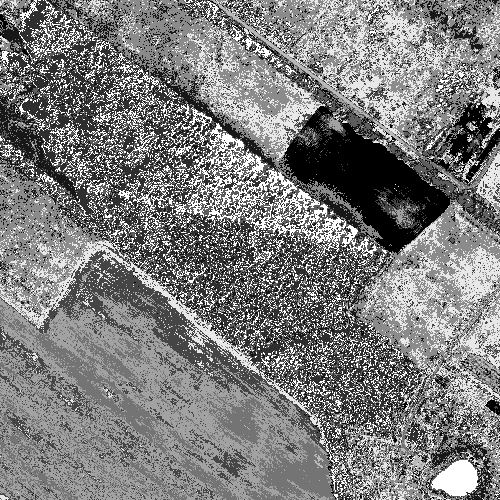
\includegraphics[width=\linewidth]{map10part}
\caption{Klašu karte ($k=12$).}
\end{subfigure}
\begin{subfigure}[b]{.3\linewidth}
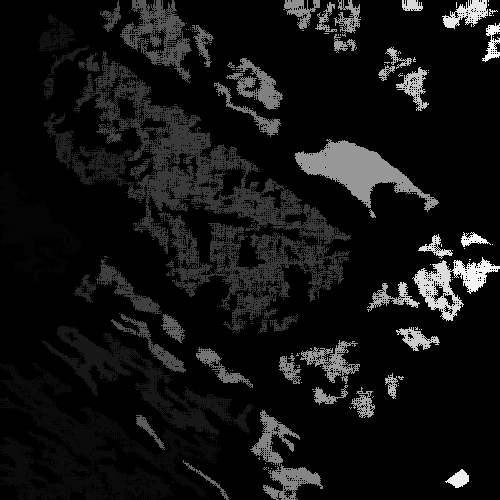
\includegraphics[width=\linewidth]{regionPecValleyD}
\caption{Identificētās ielejas.}
\label{subfig:valleyd}
\end{subfigure}
\caption{Ortofotokartes fragments ar atbilstoši identificētajām ielejām.}
\end{figure}
Kad ir atrastas ielejas (redzamas \ref{subfig:valleyd} attēlā), iespējams veikt audzēšanu lielākajā mērogā. Ieleju audzēšana pēc funkcijas \textit{ValleyG1} noris vēl arī 2. un 3. mērogā. Ievadparametri \textit{ValleyG1} funkcijai ir J-attēls \textit{JI} konkrētajā mērogā (šajā gadījumā apskatīsim \textit{JI4}) un iepriekšējā solī sagatavotā reģionu matrica apakšapgabalam \textit{subRegion} (funkcijā parametrs \textit{ValleyI}). Izvadparametrs ir arī reģionu matrica (funkcijā parametrs \textit{SegI}) tam pašam apakšapgabalam. Šīs funkcijas darbība, galvenokārt, paredzēta ieleju audzēšanai. To iespējams panākt vispirms aizpildot caurumus, kas radušies iepriekšējā fāzē. Tad atrod tos punktus no segmentētajiem, kuru vērtība mazāka par nesegmentēto punktu vidējo vērtību, bet visam attēlam no iepriekšējās fāzes \textit{ValleyI} veic atvēršanu (angl. \textit{dilation}). Pēc tam iepriekš atrastajiem punktiem, kuru vērtība mazāka par vidējo, līdzīgi, kā \textit{ValleyD} funkcijā, veic operāciju, izmantojot 4-savienojamību. Balstoties uz iegūtajiem rezultātiem pēc 4-savienojamības pielietošanas, veic ieleju audzēšanu un rezultātu pievieno \textit{SegI} matricai. Gala rezultātā atkal tiek iegūta reģionu matrica (redzama \ref{subfig:valleyg1s4ji4}). 
\begin{lstlisting}
subRegion = ValleyD(JI4,  4, mean(JI4(:)), std(JI4(:)));
subRegion = ValleyG1(JI4, subRegion);
\end{lstlisting}\par
\begin{figure}[h!]
\centering
\begin{subfigure}[b]{.3\linewidth}
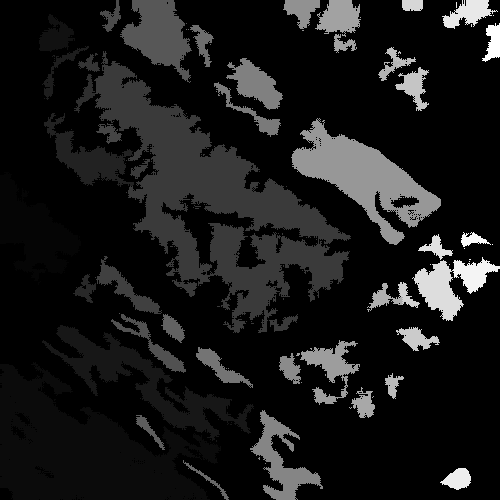
\includegraphics[width=\linewidth]{regionPecValleyG1S4JI4}
\caption{Reģioni pēc reģionu audzēšanas 4. mērogā izmantojot JI4 matricu.}
\label{subfig:valleyg1s4ji4}
\end{subfigure}
\begin{subfigure}[b]{.3\linewidth}
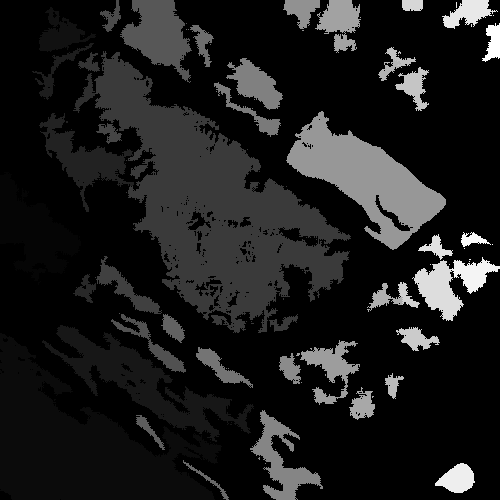
\includegraphics[width=\linewidth]{regionPecValleyG1S4JI3}
\caption{Reģioni pēc reģionu audzēšanas 4. mērogā izmantojot JI3 matricu.}
\label{subfig:valleyg1s4ji3}
\end{subfigure}
\caption{Reģionu attēli pēc audzēšanas, izmantojot funkciju \textit{ValleyG1} 4. mērogā.}
\end{figure}
Pēc tam, kad iegūta atjaunota reģionu matrica pēc reģionu audzēšanas lielākajā mērogā (izaudzētie reģioni redzami \ref{subfig:valleyg1s4ji3} attēlā), tai tiek veikta reģionu audzēšana izmantojot nākamo lielāko mērogu jeb mērogu 3 ar to pašu funkciju \textit{ValleyG1}. Kā pēdējais solis pie mēroga 4, tiek veikta ieleju audzēšana izmantojot funkciju \textit{ValleyG2}, kur atlikušie nesegmentētie punkti tiek tik daudzas reizes pārdalīti, izmantojot paša mazākā mēroga J-attēlu, līdz visi ir pieaudzēti pie kādas no ielejām.
\begin{lstlisting}
subRegion = ValleyG1(JI3, subRegion);
subRegion = ValleyG2(JI1, subRegion);
\end{lstlisting}\par
Tālāk līdzīgas darbības tiek veiktas arī nākamajos mērogos līdz galarezultātā tiek iegūta segmentēto reģionu matrica \textit{subRegion} apakšapgabalam. 
\begin{lstlisting}
% --------------------scale 3---------------------------------%
subRegion = SpatialSeg(JI3, subRegion, 3);
subRegion = ValleyG1(JI2, subRegion);
subRegion = ValleyG2(JI1, subRegion);
% --------------------scale 2---------------------------------%
subRegion = SpatialSeg(JI2, subRegion, 2);
subRegion = ValleyG1(JI1, subRegion);
subRegion = ValleyG2(JI1, subRegion);
% --------------------scale 1---------------------------------%
subRegion = SpatialSeg(JI1, subRegion, 1);
subRegion = ValleyG2(JI1, subRegion);
\end{lstlisting}\par
Tā kā katru reizi \textit{subRegion} matrica savus reģionus sāk skaitīt sākot ar 1, apakšapgabala reģionu matricas katrs reģiona numurs tiek pārvērsts tam pieskaitot šobrīd maksimālo reģiona numuru lielajā matricā \textit{region}, kurā pēc tam tāpat kā \textit{ImgQ} tiek ievietots starprezultāts apakšapgabalam.
\begin{lstlisting}
ImgQ(((i-1)*partSize)+1:endOfImV,((j-1)*partSize)+1:endOfImH, :)=partImgQ;
region(((i-1)*partSize)+1:endOfImV,((j-1)*partSize)+1:endOfImH) = subRegion;
\end{lstlisting}\par
Funkcijas \textit{mainJSEG} nobeigumā vēl tiek saglabāts \textit{subRegion} starprezultāts iepriekš izveidotajā direktorijā un cikls sāk apstrādāt nākamo apakšapgabalu. Gala rezultātā tiek atgriezta reģionu matrica \textit{region} (\textit{Region}), kas redzama attēlā \ref{fig:regionsFull} un kvantizētais attēls \textit{ImgQ} vēlākai rezultātu attēlošanai.
\begin{figure}[h!]
\centering
\begin{subfigure}[b]{.41\linewidth}
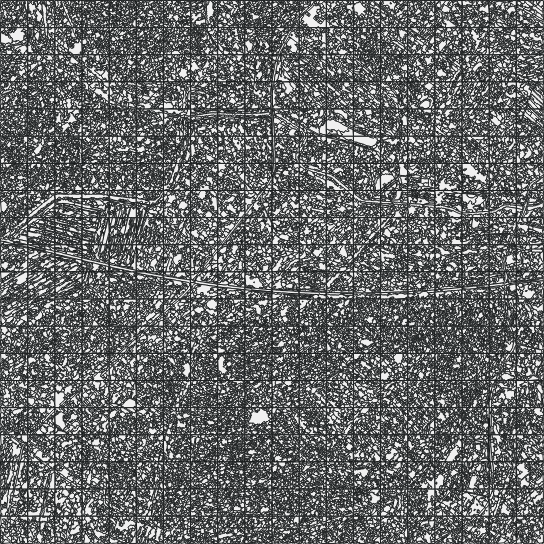
\includegraphics[width=\linewidth]{vissPolygons}
\caption{Attēls ar segmentācijas rezultātā izveidotajiem reģioniem.}
\label{fig:regionsFull}
\end{subfigure}
\begin{subfigure}[b]{.54\linewidth}
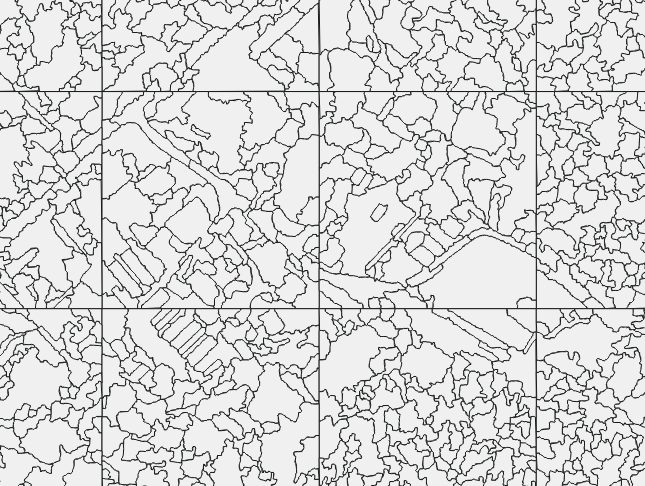
\includegraphics[width=\linewidth]{regionFragments}
\caption{Daļa no segmentācijas rezultātā izveidotajiem reģioniem. \\}
\label{fig:regionsPart}
\end{subfigure}
\caption{Segmentācijas rezultāts}
\label{fig:regions}
\end{figure}
\subsection{K-tuvāko kaimiņu metode un tās realizācija}
\subsubsection{K-tuvāko kaimiņu metodes teorētisks apskats}
K-tuvāko kaimiņu metode ir klasifikācijas metode, kas pieder pie vadītās mašīnmācīšanās metožu grupas. Klasifikācija ir sistemātiska vienumu sadalīšana grupās, kategorijās. Metodes pamatideja - pikseļa piederība kādai klasei tiek izsvērta no tā, kādai klasei pieder tā tuvākais kaimiņš. Šāds skaidrojums izmantojams gadījumā, kad $k=1$. Gadījumā, kad $k \geq 2$, piederība konkrētai klasei tiek izsvērta no lielākās daļas tuvāko kaimiņu piederības. Piemēram, gadījumā, ja $k=3$ un tiek apskatīti kāda punkta 3 tuvākie kaimiņi, kur viens no tiem pieder 1. klasei, bet divi atlikušie 2. klasei, tad apskatītais punkts pieder 2. klasei.\cite{knn} \par 
K-tuvāko kaimiņu algoritms sastāv no diviem soļiem. Pirmais solis ir tuvāko kaimiņu atrašana, bet otrais, klases piešķiršana, izmantojot šos kaimiņus.\cite{knn} \par
Lai atrastu tuvākos kaimiņus, vispirms vērts definēt jēdzienu distance. Tātad ar vārdu distance izsakām kādu mēru, kas raksturo viena pikseļa vai reģiona deskriptoru vektora attālumu līdz otram deskriptoru telpā. Iespējami vairāki veidi kā aprēķināt distances. Bieži lietota ir Eiklīda distance, kuru aprēķina
\begin{equation}
d(x,y)=\sqrt{\sum_{i=1}^{z} (x_i-y_i)^2}
\end{equation}
Šajā gadījumā $x$ un $y$ ir pikseļu vai reģionu deskriptoru vektori $z$ dimensionālā deskriptoru telpā, starp kuriem tiek aprēķināta distance. Alternatīvs un skaitļošanas ziņā ātrāks veids ir Manhetena distance. Manhetena distanci aprēķina pēc
\begin{equation}
D=\sum_{i=1}^{z}|x_i - y_i|
\end{equation}
Arī šeit $x$ un $y$ ir divi deskriptoru vektori $z$ dimensionālā deskriptoru telpā.\cite{knndistance} \par
Protams, veiksmīgi distanci iespējams aprēķināt tikai, ja deskriptoru vērtības ir normalizētas jeb visas vērtības atrodas vienā diapazonā \cite{knn}.\par
Otrais solis - klases piešķiršana, izmantojot atrastos kaimiņus ir viegli un intuitīvi saprotama gadījumā, ja $k=1$ vai $k>2$ un tuvāko kaimiņu klases nav vienādi sadalītas. Tādā gadījumā apskatītajam punktam tiek piešķirta tā klase, kāda ir visbiežāk sastopama starp kaimiņiem. Problemātiska situācija var rasties, ja $k=2$ vai klašu sadalījums starp kaimiņiem ir vienāds. Tādā gadījumā klases piešķiršana apskatītajam punktam notiek ņemot vērā kādus papildus faktorus, kā piemēram, nozīmīgāko pazīmi, ja punkts atrodas vairāku dimensiju telpā (to raksturo vairākas pazīmes), vai piešķir tieši tuvākā kaimiņa klasi. \cite{knn} \par
\subsubsection{K-tuvāko kaimiņu metodes pielietojums segmentētu reģionu klasifikācijā}
Kad visi nepieciešamie dati sagatavoti, varam sākt apskatīt funkciju \textit{classifierKNN}. Funkcija \textit{classifierKNN}, kā parametrus saņem reģionu matricu \textit{Region}, 3-dimensiju matricu attēlam \textit{image_org}, k-tuvāko kaimiņu metodes parametru \textit{k}, kas nosaka izmantoto tuvāko kaimiņu skaitu, deskriptoru matricu parauga datiem \textit{sampleDescr}, deskriptoru matricu visam attēlam \textit{vissDescr} un klašu vektoru parauga datiem \textit{sampleClasses}. Funkcijas izvadītais rezultāts ir segmentējamā attēla izmēriem atbilstoša maska, kur katra pikseļa vērtība aizstāta ar klasi, kam tas pieder. \par
Funkcija \textit{classifierKNN} izsauc funkciju \textit{mansKNN}, kas tika izstrādāta studiju kursa "\textit{Digitālo attēlu apstrāde}" ietvaros un rezultātā tiek iegūts vektors, kur katram segmentētajam reģionam atbilst tā klase. \par
Pēc tam šis vektors tiek pārvērsts klašu maskā, kas tiek atgriezta no \textit{classifierKNN} funkcijas.
\begin{lstlisting}
function mask = classifierKNN(region, rgb_image, k, sampleDescr, vissDescr, sample_classes)
	classified_image=mansKNN(vissDescr, k, sampleDescr, sample_classes);
	sample_classes=unique(sample_classes);
	[r k d]=size(rgb_image);
	mask=zeros(r,k);
	for i=1:length(classified_image)
		for j=1:length(sample_classes)
			if classified_image(i)==sample_classes(j)
				mask(region==i)=j;
			end
		end
	end
\end{lstlisting}\par
Detalizētāk apskatīsim funkciju \textit{mansKNN}, kas klasificē segmentētos reģionus. Funkcija \textit{mansKNN}, kā parametrus saņem klasificējamo attēlu \textit{im}, kas šajā gadījumā būs deskriptoru matrica visam attēlam ar deskriptoriem katram attēla segmentētajam reģionam, k-tuvāko kaimiņu metodes parametru \textit{k}, kas nosaka izmantoto tuvāko kaimiņu skaitu, parauga datus \textit{sample}, kas šajā gadījumā saturēs matricu \textit{sampleDescr} ar deskriptoru vērtībām parauga datu reģioniem un klašu vektoru parauga datiem \textit{sample_classes}. Rezultāti tiks uzglabāti matricā \textit{classIm}, kas saturēs tikpat rindiņu, cik deskriptoru matrica visiem reģioniem \textit{vissDescr}.\par
Pati funkcija tikai izveido matricu rezultāta uzglabāšanai un ciklā katram reģionam nosaka tā piederību konkrētai klasei izmantojot funkciju \textit{knnProcedura}.
\begin{lstlisting}
function classIm=mansKNN(im,k,sample,sample_classes)
    [r, ko, d]=size(im);
    classIm=zeros(r,1);
    for i=1:r
        x=im(i,:);
        classIm(i)=knnProcedura(x,sample,sample_classes,k);
    end
\end{lstlisting}\par
Funkcija \textit{knnProcedura}, kā parametrus saņem reģiona deskriptoru vektoru x, deskriptoru matricu parauga datiem \textit{sample}, parauga datu klašu vektoru \textit{sample_classes} un k-tuvāko kaimiņu metodes parametru \textit{k}. Vispirms tiek noteikt parauga datu skaits un izveidots vektors \textit{d}, kas sevī saturēs distances no reģiona, kam tiek meklēta klases piederība līdz visiem pārējiem parauga datu reģioniem.
\begin{lstlisting}
function knnResponse=knnProcedura(x,sample,sample_classes,k)
    sampleN=length(sample_classes);
    d=zeros(sampleN,1);
    for z=1:sampleN
        d(z)=sqrt(sum((x-sample(z,:)).^2));
    end
\end{lstlisting}\par
Kad atrastas visas distances nepieciešams noteikt \textit{k} īsākās. To realizē ciklā aizpildot \textit{k} garu rindas vektoru ar tām distancēm atbilstošo reģionu klasēm, kas ir vismazākās un šo distanču vērtības aizvietojot ar bezgalību, lai visās \textit{k} reizēs netiktu atrasta viena vērtība. Pēc tam no šīm \textit{k} klasēm tiek noteikta vektora moda jeb vērtība, kas atkārtojas visbiežāk, kas arī tiek atgriezta, kā rezultāts funkcijai \textit{knnProcedura}.
\begin{figure}[h!]
\centering
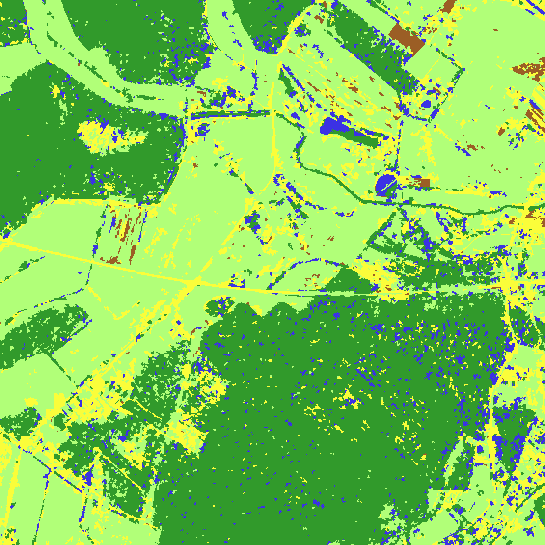
\includegraphics[width=.6\linewidth]{result}
\caption{Klašu maska klasificētajiem JSEG segmentācijas rezultātiem, izmantojot k-tuvāko kaimiņu metodi.}
\label{fig:resultKNN}
\end{figure}
\begin{lstlisting}
    typesForKNb=zeros(1,k);
    for z=1:k
        [m, I]=min(d);
        typesForKNb(z)=sample_classes(I);
        d(I)=Inf;
    end
    knnResponse=mode(typesForKNb);
\end{lstlisting}\par
\ref{fig:resultKNN} attēlā redzama klašu maska pēc reģionu klasifikācijas, izmantojot k-tuvāko kaimiņu metodi. Zilā krāsā attēloas ūdens platības, tumši zaļā - koku pārsegums, gaiši zaļā - zālāji, brūnā - lauki un dzeltenā krāsā platības, kas atbilst citam pārseguma tipam.
\section{Neironu tīklu pielietojums}
\subsection{Apmācības datu sagatavošana} \label{ssec:apmDati}
Apmācības datu sagatavošanai tiek izmantoti tie paši attēli mazākā apjomā kā k-tuvāko kaimiņu metodes gadījumā. Ja k-tuvāko kaimiņu metodes gadījumā, lai aprēķinātu deskriptorus, bija iespējams izmantot reģionu attēlus katram pārseguma tipam tos iepriekš nekā neapstrādājot, tad neironu tīkla pielietošanas gadījumā situācija ir citādāka. Šajā gadījumā reģionu attēlus nepieciešams sadalīt smalkāk jeb tā, ka katrs reģions ir atsevišķs attēls. \par
Lai sasniegtu šādu rezultātu un izvairītos no nevēlamu artifaktu parādīšanās attēlos, ar programmatūras \textit{MatLab} palīdzību tika izveidota funkcija \textit{saveTestDataByRegion}. Šī funkcija, kā ievadparametrus saņem matricu \textit{testRegion} ar tā pārseguma tipa parauga datu reģioniem, ko nepieciešams sadalīt attēlos, oriģinālā attēla matricu \textit{I} ciparu formātā \textit{double} formā $ M \times N \times 3 $, kur $ M $ apzīmē rindiņu skaitu, bet $ N $ - kolonnu skaitu un pārseguma tipa kārtas numuru \textit{folder} direktorijas izveidošanai, kur tiks saglabāti izveidotie attēli. Vispirms tiek atrasti to reģionu numuri, kurus satur matrica \textit{testRegion} un izveidota direktorija izveidoto attēlu saglabāšanai.
\begin{lstlisting}
function saveTestDataByRegion(testRegion, I, folder)
	uniqueRegions=unique(testRegion);
	mkdir(in2str(folder));
\end{lstlisting}\par
Tālāk ciklā, ejot cauri unikālajiem reģionu numuriem sākot no otrā, jo pirmais vienmēr apzīmēs visus tos reģionus, kas nepieder izvēlētajiem parauga datiem, izveido matricu \textit{region}, kas saturēs tajā brīdī apskatāmo reģionu. Izmantojot \textit{MatLab} iebūvēto funkciju \textit{regionprops}, tiek atrasti mazākie taisnstūri, kas iekļauj apskatītajā reģionā savienotus objektus un informācija par šiem taisnstūriem tiek saglabāta mainīgajā \textit{stats}. Pēc tam, ja mainīgais \textit{stats} sevī ietver vairāk kā vienu savienoto komponenti ar to aptverošo taisnstūri, tiek izveidots rindas vektors \textit{sizes}. Izmantojot ciklu, šis rindas vektors tiek aizpildīts ar komponenti aptverošā taisnstūra rindu un kolonnu skaita summu. Balstoties uz šo aptverošo taisnstūru izmēriem, tiek paturēta lielākā komponente, kuru aptverošā taisnstūra augšējā kreisā stūra koordinātas un rindas un kolonnu skaits tiek padots kā vektors tālākai apstrādei. Ja eksistē tikai viena savienotā komponente,  tās aptverošā taisnstūra parametri tiek padoti tālāk.
\begin{lstlisting}
    for i=2:length(uniqueRegions)
        region=(testRegion==uniqueRegions(i));
        stats=regionprops(region,'BoundingBox');
        if(length(stats)>1)
            sizes=zeros(1,length(stats));
            for j=1:length(stats)
                bb=ceil(stats(j).BoundingBox);
                sizes(j)=bb(3)+bb(4);
            end
            [M idx]=max(sizes);
            bb=ceil(stats(idx).BoundingBox);
        else
            bb=ceil(stats(1).BoundingBox);
        end
\end{lstlisting}\par
Lai izvairītos no smalku un līdz ar to nederīgu reģionu saglabāšanas, pārbauda, vai aptverošā taisnstūra laukums ir lielāks par 80 pikseļiem. Ja aptverošā taisnstūra laukums nesasniedz 80 pikseļus, cikls šajā momentā tiek pārtraukts un attiecīgais reģions kā attēls saglabāts netiek. Šādos smalkos reģionos parādās nekorektas un realitātei neatbilstošas pikseļu un reģionu raksturojošo parametru (vidējās vērtības, mediānas, standartnovirzes) vērtības, kas var negatīvi ietekmēt apmācības gaitu.
\begin{lstlisting}
        if(bb(3)*bb(4)<80)
            continue;
        end
\end{lstlisting}\par
Kad iegūtas derīga reģiona kreisā augšējā stūra koordinātas un izmēri, tos izmantojot no reģionu un oriģinālā attēla, tiek atlasītas matricas, kuru reizinājums tiek saglabāts, kā attēls \textit{JPEG} formātā iepriekš noteiktā direktorijā.
\begin{lstlisting}
		croppedRegion=region(bb(2):bb(2)+bb(4)-1,bb(1):bb(1)+bb(3)-1);
        croppedIm=I(bb(2):bb(2)+bb(4)-1,bb(1):bb(1)+bb(3)-1,:);
        result=croppedRegion.*croppedIm;
        imwrite(result,[in2str(folder) '/' int2str(uniqueRegions(i)) '.jpg'],'jpg');
    end
\end{lstlisting}
\begin{figure}[h!]
\centering
\begin{subfigure}[b]{.32\linewidth}
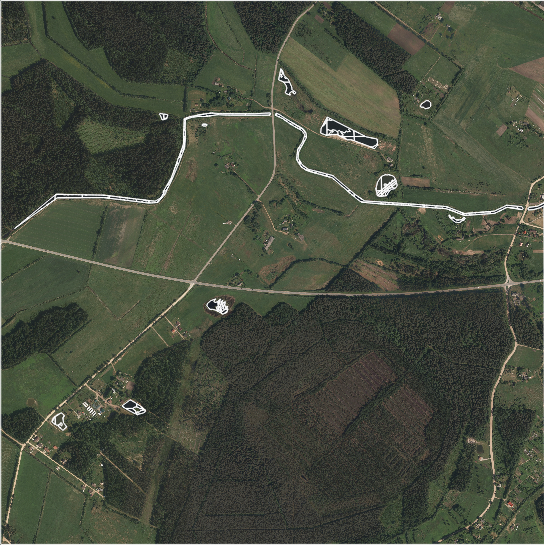
\includegraphics[width=\linewidth]{udensSampleNN}
\caption{Ūdens parauga dati.}\label{fig:udensSampleNN}
\end{subfigure}
\begin{subfigure}[b]{.32\linewidth}
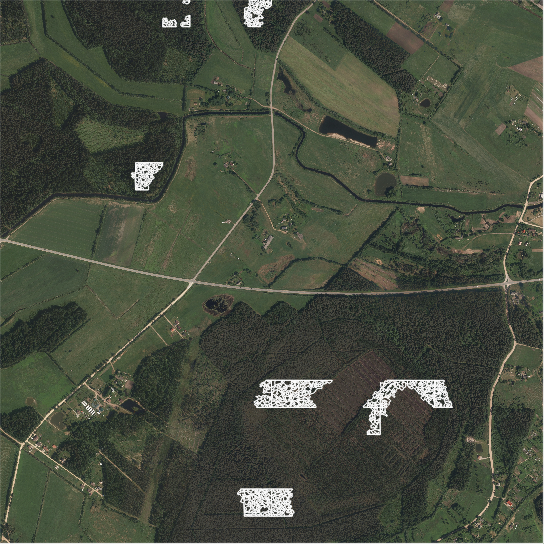
\includegraphics[width=\linewidth]{kokiSampleNN}
\caption{Koku parauga dati.}\label{fig:kokiSampleNN}
\end{subfigure}
\begin{subfigure}[b]{.32\linewidth}
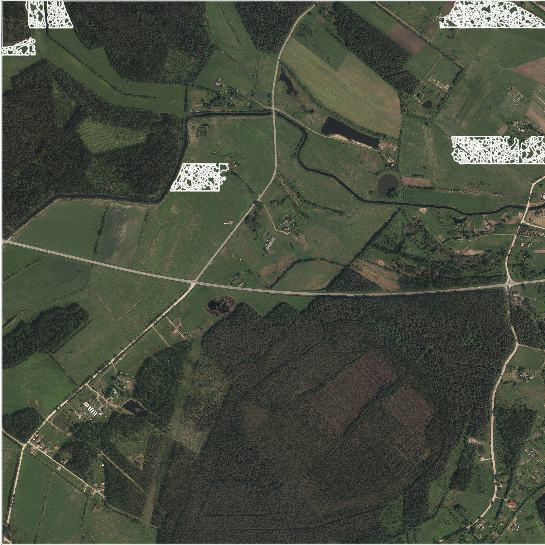
\includegraphics[width=\linewidth]{zaliensSampleNN}
\caption{Zāliena parauga dati.}
\label{fig:zaliensSampleNN}
\end{subfigure}
\begin{subfigure}[b]{.32\linewidth}
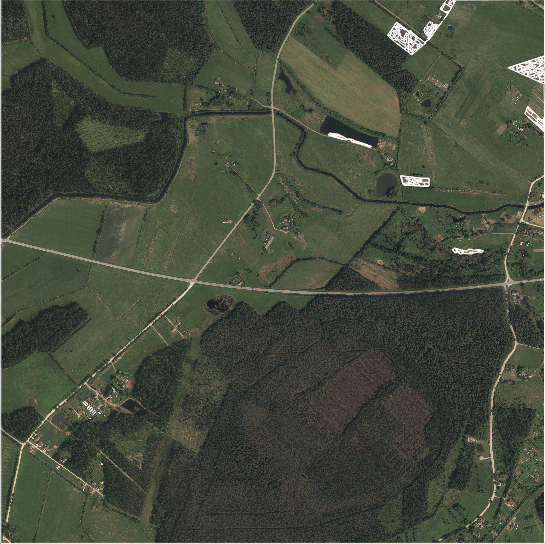
\includegraphics[width=\linewidth]{lauksSampleNN}
\caption{Lauku parauga dati.}\label{fig:lauksSampleNN}
\end{subfigure}
\begin{subfigure}[b]{.32\linewidth}
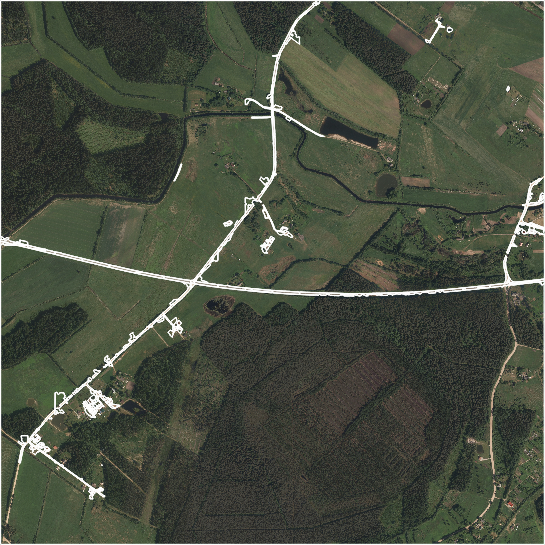
\includegraphics[width=\linewidth]{citsSampleNN}
\caption{Citi parauga dati.}\label{fig:citsSampleNN}
\end{subfigure}
\label{fig:sampleNN}
\caption{Parauga dati neironu tīkla apmācībai.}
\end{figure}\par
Izpildot šo funkciju katra zemes pārseguma tipa parauga datu reģionu failam, galarezultātā tiek iegūtas 5 direktorijas ar attiecīgajiem parauga datiem tajās. Lai vienlīdz labi apmācītu neironu tīklu atpazīt visas zemes pārseguma tipu klases, "\textit{zāliena}" un "\textit{koku}" klasei apmācības datu skaits tiek samazināts līdz 1000 attēliem. Bez "\textit{zāliena}" (attēls \ref{fig:zaliensSampleNN}) un "\textit{koku}" (attēls \ref{fig:kokiSampleNN}) parauga datiem neironu tīkla apmācībai tiek izmantoti 284 attēli ar "\textit{ūdens}" (attēls \ref{fig:udensSampleNN}) parauga datu reģioniem, 336 attēli ar "\textit{lauku}" (attēls \ref{fig:lauksSampleNN}) parauga datu reģioniem un 365 attēli ar "\textit{cita}" parauga datu reģioniem.
\subsection{Neironu tīkla teorētisks apskats}
\subsubsection{Bioloģiskie un mākslīgie neironi un tīkli}
Mākslīgie neironu tīkli (LZA, angl. \textit{artificial neural networks}) ir pētīti jau vairākus desmitus gadu, lai spētu iegūt līdzīgus rezultātus balss un attēlu atpazīšanā kā izmantojot cilvēka maņu orgānus un smadzenes. Lai arī datoru skaitļošanas jaudas šobrīd ir kļuvušas spēcīgākas kā vēl nekad, joprojām cilvēka smadzenēm vieglāk padodas tādu uzdevumu atrisināšana, kā veselo augļu atšķiršana no bojātajiem un negataviem vai arī seju atpazīšana.\cite{NNIntroduction1987},\cite{NNforHyperspectralIm2010},\cite{zutersNeironuTikli}\par
Mākslīgie neironu tīkli ir informācijas apstrādes sistēmas, kas sastāv no liela skaita skaitļošanas vienību (neironu). To izveide ir balstīta uz pētījumiem par cilvēka smadzeņu un nervu sistēmas darbību. Mākslīgo neironu tīklu mērķis ir izveidot skaitļošanas sistēmu, kas būtu līdzīga cilvēka smadzenēm - kompleksa, paralēla un nelineāra. \cite{krose1993introduction} \par
Neironu tīklu veido liels skaits savā starpā cieši saistītu informācijas apstrādes elementu jeb neironu, kas kopā veic konkrētu uzdevumu vai atrisina konkrēto problēmu. Mākslīgo neironu tīklu var arī saukt par vispārīgu cilvēka smadzeņu modeli, lai arī tas no cilvēka smadzenēm spējis adaptēt tikai divas īpašības:
\begin{itemize}
\item Spēju tikt apmācītam jeb veids, kā neironu tīkls iegūst informāciju un zināšanas.
\item Savienojamību jeb tas, cik ļoti stipras saites pastāv starp neironiem nosaka to, kā tīklā tiek uzglabātas zināšanas.\cite{zutersNeironuTikli}\par
\end{itemize}
Mākslīgā neironu tīkla iespējas slēpjas tā neironos un to saitēs. Lai arī viens pats mākslīgais neirons ir tikai salīdzinoši vienkārša skaitļošanas vienība, liels to daudzums un veidi, kā tie ir savienoti palīdz atrisināt dažādus uzdevumus. Salīdzinoši ar bioloģiskajiem neironiem, kas atrodami cilvēka smadzenēs, mākslīgo neironu takts frekvence ir daudz augstāka, bet toties to skaits ir daudz mazāks, kas rada bažas vai jebkad mākslīgie neironu tīkli spēs risināt tādus pašus uzdevumus, kā cilvēka smadzenes.\cite{zutersNeironuTikli}\par
Ņemot vērā, ka mākslīgo neironu tīkla ideja ir aizgūta no bioloģiskajiem neironu tīkliem, vērts apskatīt bioloģiskā neirona uzbūvi. Cilvēka smadzenes sastāv no aptuveni 10 miljardiem neironu un katrs no tiem ir savienots ar 10 tūkstoš citu neironu. Neirons jeb nervu šūna sastāv no:
\begin{itemize}
\item ķermeņa jeb somas (angl. \textit{soma});
\item tieviem, mugurkaulam līdzīgiem ar izteiktiem sazarojumiem izaugumiem - dendrītiem (angl. \textit{dendrites}); 
\item resnāka izauguma, kas savienojas ar citiem neironiem - aksona (angl. \textit{axon}).
\end{itemize}
Neirons informāciju iegūst, izmantojot sinapses (angl. \textit{synapses}) pirms tā tiek novadīta aksonam. \cite{dennis1997introduction}
\begin{figure}[h!]
\centering
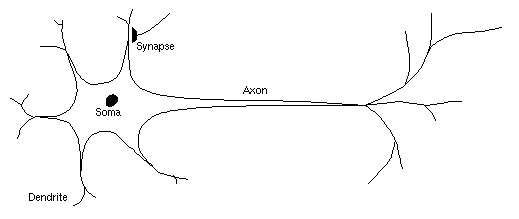
\includegraphics[width=.7\linewidth]{neuron}
\label{fig:neuron}
\caption{Bioloģiskā neirona shematisks zīmējums \cite{dennis1997introduction}.}
\end{figure}\par
Mākslīgā un bioloģiskā neirona līdzība saskatāma jau tajā, ka mākslīgais neirons no bioloģiskā ir aizguvis vairākas īpašības, kā piemēram:
\begin{itemize}
\item neironā norisinās ienākošo vērtību svērtā summēšana;
\item neironā ienāk vairāki signāli;
\item uztverošās sinapses svars var veikt neironā ienākošās vērtības izmaiņas;
\item aksonam raksturīga sazarošanās, tātad neirona izejas vērtība var nonākt vairākos citos neironos;
\item gadījumā, kad ievads ir pietiekams, neirons izejā var dot tikai vienu signālu.
\end{itemize}
Papildus šīm īpašībām mākslīgajiem neironiem ir arī īpašības, kas aizgūtas balstoties uz bioloģiskajiem neironiem, kā piemēram:
\begin{itemize}
\item neironā atmiņa ir sadalīta;
\item īslaicīgā atmiņa ir signāli, kurus izsūta neironi;
\item ilglaicīgā atmiņa atrodas neironu sinapsēs;
\item svarus sinapsēs var mainīt balstoties uz pieredzi;
\item sinapsēm var būt gan pastiprinoša, gan pavājinoša iedarbība;
\item informācija tiek apstrādāta lokāli. \cite{fausett1994}
\end{itemize}\par
Tā kā vispārīgā gadījumā neironu tīkls sastāv no liela skaita neironu, var uzskatīt, ka neirons ir salīdzinoši vienkārša neironu tīkla sastāvdaļa. Tā kā neironu tīklā galvenā loma ir nevis konkrētām tā sastāvdaļām, bet gan neironu savstarpējam novietojumam, neironu tīklu ir grūti vispārīgi modelēt, testēt un lietot. Tieši šī īpašība neironu tīklu nepadara par unikālu visu problēmu atrisinājumu. Lielā daļā problēmu joprojām labākus rezultātus sasniedz standarta algoritmi. Neironu tīklu kā risinājumu problēmai tā sarežģītās struktūras dēļ vērts izmantot problēmu risināšanai, kur parastā standarta pieeja nesniedz gaidīto rezultātu jeb ir neefektīva. Otrs variants, kad vērts apsvērt neironu tīkla izmantošanu, ir gadījumos, kad informācija par problēmu nav pilnīga. Par spīti tam, ka par neironu tīklu var spriest tikai, ja tam ir daudz elementu, ir vērts aplūkot arī atsevišķa neirona uzbūvi, jo tā var būtiski ietekmēt skaitļošanas jaudu. \cite{zutersNeironuTikli}\par
Mākslīgais neirons sastāv no svariem, summēšanas jeb izplatīšanas funkcijas un aktivitātes funkcijas. Tā shēma un galvenās sastāvdaļas redzamas \ref{fig:artificialNeuron} attēlā, bet katru no sastāvdaļām apskatīsim smalkāk.
\begin{figure}[h!]
\centering
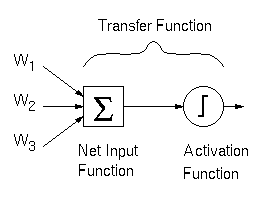
\includegraphics[scale=0.85]{transfer}
\caption{Mākslīgā neirona shematisks zīmējums \cite{dennis1997introduction}.}
\label{fig:artificialNeuron}
\end{figure}\par
Svari, saukti arī par sinaptiskiem svariem (angl. \textit{synaptic weights}) ir vērtības, ar kuru palīdzību neironā ienākošais signāls tiek izmainīts. Svari lielā mērā nosaka to, cik ļoti neirons atšķiras no neirona, jo visam neironu tīklam vai atsevišķai neironu grupai izplatīšanās un aktivitātes funkcijas parasti ir vienādas. Tāpat arī svari ir atbildīgi par neironu tīkla mācīšanās spēju, jo tos mainot iespējams pielāgot neironu tīklu atrisināt konkrētu problēmu. Parasti svaru skaits atbilst ieeju skaitam, bet var būt arī viens papildus svars. Svarus no angļu valodas vārda \textit{weight} apzīmē ar burtu \textit{w} un indeksu, kas parāda ieejas kārtas numuru. Visu svaru apzīmēšanai izmanto matricu pierakstu ($w$ vai $W$).\cite{zutersNeironuTikli}\par
Summēšanas funkcija (angl. \textit{propagation function}) ir atbildīga par visu ienākošo signālu kombinēšanu ar to svariem un kopējās vērtības padošanu tālāk aktivitātes funkcijai. Parasti izmanto signālu un to atbilstošo svaru reizinājumu summu kā summēšanas funkciju. Šīs funkcijas aprēķināto vērtību parasti apzīmē ar burtu virkni $NET$.\cite{zutersNeironuTikli}\par
Aktivitātes funkcija ir svarīgākā neirona darbības raksturotāja. Aktivitātes funkcija nosaka to, kāda tipa problēmu risinās neirons. Pati funkcija, izmantojot summēšanas funkcijas galarezultāta vērtību $NET$, aprēķina izejas vērtību.\cite{zutersNeironuTikli}
\subsubsection{Konvolucionālie neironu tīkli}
Konvolucionālais neironu tīkls (angl. \textit{convolutional neural network}) ir īpašs mākslīgo neironu tīkla veids, ko bieži izmanto plašā spektrā tēlu pazīšanas problēmu, kā piemēram, datorredzē (angl. \textit{computer vision}), runas pazīšanā (LZA, angl. \textit{speech recognition}) un citur. Turpmākajā aprakstā apskatīsim tikai divdimensionālus konvolucionālos neironu tīklus. Konvolucionālā neironu tīkla galvenā ideja ir veidot invariantas īpašības neironu tīkliem, veidojot tādus modeļus, kas arī ir invarianti noteiktiem ievades datu pārveidojumiem. Ideja ir radusies no problēmas, kas ir bieži sastopama vienvirziena neironu tīklos (angl. \textit{feed forward neural networks}) un it īpaši vairākslāņu vienvirziena neironu tīklos. Problēma ir tajā, ka vairākslāņu vienvirziena neirona tīklam slāņi savā starpā ir savienoti un tas noņem ievades telpisko informāciju, kas nepieciešama aprēķiniem.\cite{fukushima1982}\par
Atšķirībā no parastajiem neironu tīkliem, konvolucionālajiem neironu tīkliem ir īpaša arhitektūra. Arhitektūra parasti sastāv no konvolucionālā slāņa un apakšparauga atlases slāņa (LZA, angl. \textit{sub-sampling layer}) kā redzams attēlā \ref{fig:architecture}.
\begin{figure}[h!]
\centering
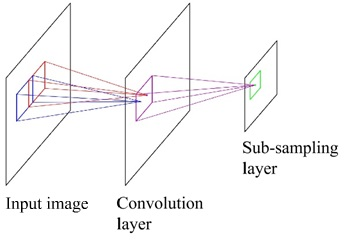
\includegraphics[width=.5\linewidth]{convArchitecture}
\caption{Konvolucionālā neironu tīkla arhitektūra \cite{convolutionalNN}.}
\label{fig:architecture}
\end{figure}
Konvolucionālais slānis implementē konvolūcijas operāciju un apakšparauga atlases operācija norisinās apakšparauga atlases slānī. Konvolucionālie neironu tīkli ir veidoti balstoties uz trīs galvenajām idejām - vietējiem uztverošajiem laukumiem, svaru dalīšanu un apakšparaugu atlasi jeb savstarpēju izmantošanu (LZA, angl. \textit{pooling}). Katru ideju apskatīsim sīkāk. \cite{convolutionalNN}\par
\begin{figure}[h!]
\centering
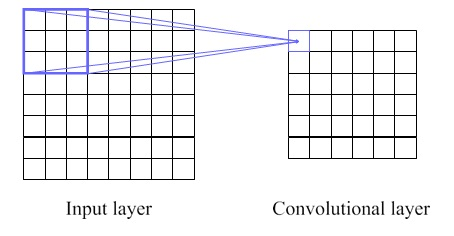
\includegraphics[width=.6\linewidth]{localReceptiveField}
\caption{Vietējā uztverošā laukuma piemērs konvolucionālajā slānī \cite{convolutionalNN}.}
\label{fig:localReceptiveField1}
\end{figure}
\paragraph{Vietējie uztverošie laukumi}Vienvirziena neironu tīklā ievade ir cieši saistīta ar nākamo slēpto mezglu katram neironam. Turpretī konvolucionālā neironu tīklā ievade veido savienojumus tikai mazā reģionā. Katrs neirons slēptajā slānī būs savienots tikai ar mazu laukumu no iepriekšējā slāņa, ko sauc par vietējo uztverošo laukumu. \ref{fig:localReceptiveField1} attēlā ar violeto kvadrātu apzīmēts vietējais uztverošais laukums, bet ar violetajām līnijām, kā tas savienots ar neironu. \cite{convolutionalNN}
\paragraph{Svaru dalīšana} Konvolūcionālajā slānī neironi ir izkārtoti vairākos paralēlos slēptajos slāņos jeb iezīmju kartēs (angl. \textit{feature map}). Katrs neirons iezīmju kartē ir savienots ar vietējo uztverošo laukumu. Katrai iezīmju kartei visi neironi dala vienu un to pašu svara parametru, kas ir pazīstams kā filtrs.\cite{convolutionalNN}
\paragraph{Savstarpējā izmantošana} Konvolucionālais neironu tīkls satur ne tikai konvolucionālos slāņus, bet dažreiz arī savstarpējās izmantošanas slāņus (angl. \textit{pooling layers}). Gadījumos, kad šis slānis eksistē, to parasti izmanto uzreiz pēc konvolucionālā slāņa. Tas nozīmē, ka konvolucionālā slāņa izvads ir ievads savstarpējās izmantošanas slānī. Šis slānis ir paredzēts, lai ģenerētu translācijas invarianta iezīmes, aprēķinot statistiku no konvolūciju aktivācijas mazam uztveršanas laukumam, kas atbilst iezīmju kartei. Šeit mazā uztverošā laukuma izmērs ir atkarīgs no savstarpējās izmantošanas izmēra. \ref{fig:pooling3} attēlā redzams, kā savstarpējās izmantošanas slānis darbojas katrai iezīmju kartei.\cite{convolutionalNN}
\begin{figure}[h!]
\centering
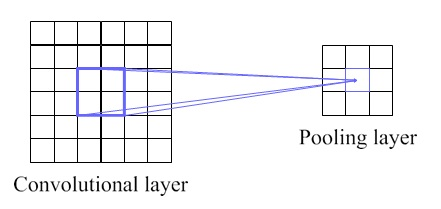
\includegraphics[width=.6\linewidth]{pooling}
\caption{Savstarpējās izmantošanas slāņa piemērs iezīmju kartei \cite{convolutionalNN}.}
\label{fig:pooling3}
\end{figure}
\subsubsection{Bibliotēka \textit{Tensorflow} un \textit{Inception} modelis} \textit{TensorFlow} ir atvērtā koda mašīnmācīšanās metožu bibliotēka. Skaitļošanu, kas veikta izmantojot \textit{TensorFlow}, iespējams izpildīt ar nelielām vai bez izmaiņām uz dažādām sistēmām, sākot ar mobilām ierīcēm līdz pat plaša mēroga dalītām sistēmām, kas sastāv no simtiem mašīnu un tūkstošiem skaitļošanas vienību. Fakts, ka eksistē viena sistēma, kas noklāj tik plašu platformu loku, ievērojami atvieglo reālās dzīves pielietojumu mašīnmācīšanās sistēmām. Sistēmu ir viegli pielāgot un to var izmantot, lai izteiktu dažādus algritmus, veiktu pētījumus un uzstādītu mašīnmācīšanās sistēmas produkcijas vidē vairāk kā desmit datorzinātņu nozarēs, ieskaitot runas pazīšanu, datorredzi, robotiku, informācijas izguvi, dabīgo valodu apstrādi, ģeogrāfiskās informācijas izdalīšanu un citās. \cite{tensorflow}\par
\textit{Google Brain} projekts sākās 2011. gadā ar mērķi izpētīt ļoti plaša mēroga dziļās apmācības neironu tīklu pielietojumu izpētē un, lai izmantotu \textit{Google} produktos. Viens no pirmajiem produktiem projekta ietvaros tika izveidots \textit{DistBelief} - pirmās paaudzes mērogojama, sadalīta apmācības un secinājumu sistēma. Balstoties uz pieredzi, kas gūta, strādājot ar \textit{DistBelief} un lielāku sapratni par vēlamās sistēmas īpašībām un prasībām apmācībai un neironu tīkla izmantošanā, tika radīts \textit{TensorFlow} - otrās paaudzes sistēma implementācijai un plaša mēroga mašīnmācīšanās modeļu uzstādīšanai. \cite{tensorflow}\par
\textit{TensorFlow} ir atvērtā koda programmatūras bibliotēka cipariskām skaitļošanām, izmantojot datu plūsmas grafus (LZA, angl. \textit{data flow graph}). Mezgli grafos apzīmē matemātiskās operācijas, bet grafu malas daudzdimensionālus datu masīvus (tenzorus), kas starp mezgliem plūst. \cite{tensorflow}\par
\begin{figure}[h!]
\centering
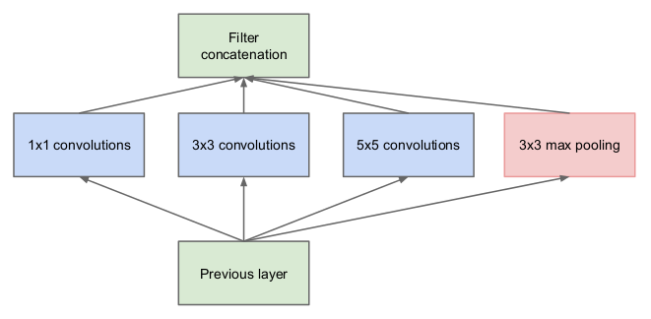
\includegraphics[width=.7\linewidth]{inception1}
\label{fig:inception1}
\caption{\textit{Inception} modulis \cite{inception}.}
\end{figure}
Viens no \textit{TensorFlow} iekļautajiem modeļiem ir \textit{Inception} modelis. \textit{Inception} modeļa arhitektūras galvenā pamatideja ir balstīta uz to retināta struktūra konvolucionālā redzamības tīklā var tikt tuvināti nosegta ar blīvām komponentēm. Viss, kas ir vajadzīgs, ir atrast optimālu vietējo konstrukciju un to telpiski atkārtot. Viens no risinājumiem ir konstrukcija slāni pa slānim, kur būtu jāanalizē korelācijas statistika pēdējam slānim un tad pudurot tos grupās ar augstu korelāciju. Šie puduri veidos nākamā slāņa vienības un būs savienoti ar iepriekšējo slāni. Varam pieņemt, ka katra vienība no iepriekšējā slāņa atbilst kādam reģionam no ievadattēla un šīs vienības ir sagrupētas filtru bankās. Zemākajos slāņos jeb tajos, kas tuvāki ievadei, korelētās vienības veidotu vietējos reģionus. Tas nozīmē, ka beigās tiktu iegūts daudz koncentrētu puduru vienā reģionā un tos iespējams noklāt ar $1 \times 1$ konvolūcijām nākamajā slānī.\cite{inception}\par
\begin{figure}[h!]
\centering
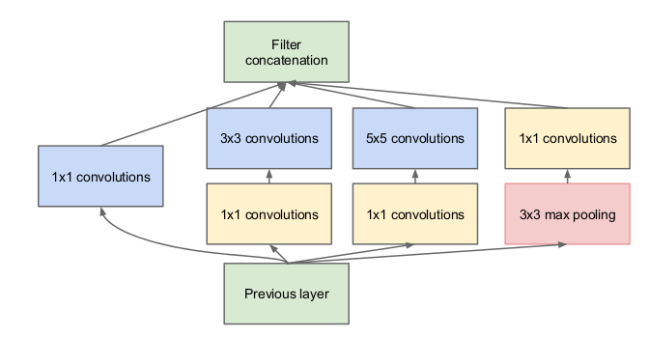
\includegraphics[width=.7\linewidth]{inception2}
\label{fig:inception2}
\caption{\textit{Inception} modulis ar dimensiju skaita samazināšanu \cite{inception}.}
\end{figure}
Lai izvairītos no problēmām, kas rodas apgabalu salāgošanas dēļ, tagadējās \textit{Inception} arhitektūras iemiesojumi izmanto $1 \times 1$, $3 \times 3$ un $5 \times 5$ filtru izmērus. Tas arī nozīmē, ka ieteiktā arhitektūra ir visu slāņu un to izvades filtru banku kombinācija apvienota vienā izvades vektorā, kas veido nākamā līmeņa ievadi. Visu apkopojot, \textit{Inception} tīkls ir tīkls, kas sastāv no augstāk aprakstītā tipa moduļiem, izvietotiem viens virs otra, ar laiku pa laikam esošiem  maksimālas savstarpējās izmantošanas slāņiem ar soli sākot no divi līdz pusei no tīkla izšķirtspējas. \cite{inception}\par
\subsection{Neironu tīkla izmantošana JSEG reģionu klasifikācijai}
Nākamais solis aiz parauga datu sagatavošanas JSEG segmentācijas rezultātu klasifikācijā ir mākslīgā neironu tīkla apmācība. Kā pamats tiek ņemts repozitoriju uzglabāšanas platformā \textit{GitHub}, \textit{TensorFlow} projekta, \textit{Tensorflow} repozitorijā esošais, brīvi pieejamais kods, kas paredzēts \textit{Inception} modeļa pēdējā slāņa vairākkārtējai apmācībai attēlu klasifikācijā un klašu piešķiršanai klasificējamiem attēliem.\par
\textit{Inception} modelis ir jau iepriekš apmācīts attēlu klasificēšanā un katru reizi, apmācot tā pēdējo slāni, iespējams modelim iemācīt atpazīt jaunas attēlu klases. Šāda pieeja ne tikai ievērojami saīsina apmācības laiku no vairākām nedēļām līdz nepilnai stundai, bet arī sniedz pārsteidzoši labus rezultātus. Modelis ir pilnībā apmācīts, izmantojot attēlus no \textit{ImageNet} attēlu datu kopas. Lai atkārtoti apmācītu pēdējo modeļa slāni, nepieciešama direktorija, kas satur apakšdirektorijas ar parauga datiem. Īpaša uzmanība jāpievērš apakšdirektoriju nosaukumiem, jo tieši tie nosaka atpazīstamo klašu nosaukumus. \ref{ssec:apmDati} apakšnodaļā jau apskatījām, kā izveidot parauga datu attēlus ar atbilstošajām apakšdirektorijām.
\begin{figure}[h!]
\centering
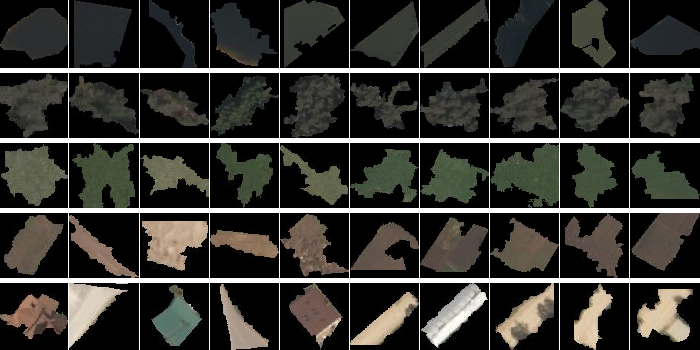
\includegraphics[width=\linewidth]{paraugaDatiTF}
\caption{Zemes pārseguma tipu parauga datu attēli.}
\label{fig:paraugaDati}
\end{figure}
Jāpiebilst, ka parauga datu attēlu nosaukumi nav svarīgi, tādēļ šajā gadījumā attēlu nosaukumi atbilst to reģionu kārtas numuriem, kas radušies JSEG segmentācijas rezultātā. Attēlā \ref{fig:paraugaDati} redzami daži no apmācībā izmantotiem attēliem - 1. rindā ūdens pārseguma tipam, 2. rindā koku pārseguma tipam, 3. rindā zāliena pārseguma tipam, 4. rindā lauku pārseguma tipam un 5. rindā citam pārseguma tipam.\par
Apmācībā un attēlu klasificēšanā nepieciešams uz darbsistēmas instalēt programmēšanas valodu \textit{Python}. Lai \textit{TensorFlow} bibliotēka sekmīgi tiktu importēta, nepieciešams instalēt vismaz  \textit{Python 3.5.2} versiju. Tāpat veiksmīgai apmācības un klasificēšanas skriptu izpildei nepieciešams papildus instalēt bibliotēkas \textit{numpy+mkl} un \textit{scipy}. Lai veiktu apmācību, no komandrindas, atrodoties direktorijā, kur pieejams brīvi pieejamais atvērtā koda \textit{Python} skripts \textit{retrain.py}, šo skriptu izpilda. Kā parametrs skripta izpildē tiek padots apakšdirektorijas nosaukums, kur saglabātas direktorijas ar parauga datiem.
\begin{lstlisting}[language=bash]
python retrain.py --image_dir paraugaDati
\end{lstlisting}\par
Pēc veiksmīgas modeļa pēdējā slāņa otrreizējas apmācības iespējams veikt JSEG segmentācijas rezultātā radušos reģionu klasifikāciju. Līdzīgi, kā apmācības datu sagatavošanā, arī segmentēto ortofotokarti nepieciešams sadalīt atsevišķos attēlos katram reģionam. Lai to īstenotu, izmanto \ref{ssec:apmDati} apakšnodaļā minēto funkciju \textit{saveTestDataByRegion}, pirms tam to attiecīgi pielāgojot. Kā pirmais pielāgojums minams cikla sākšana ar pirmo elementu, jo atšķirībā no parauga datu reģionu attēlu sagatavošanas, segmentētās ortofotokartes reģionu attēlā nav nulles vērtības. Otrs pielāgojums saistīts ar nosacījuma bloka dzēšanu, kas atbild par mazo laukumu (mazāki par 80 pikseļiem) neiekļaušanu parauga datos. Tā kā nepieciešams klasificēt visus reģionus, šis nosacījuma bloks tiek dzēsts. Pēc augstāk minētās funkcijas izpildes tiek izveidota direktorija, kas satur visus reģionu attēlus. Pēc tam šo direktoriju pārvieto uz to direktoriju, kur atrodas brīvi pieejamais atvērtā koda \textit{Python} skripts \textit{label_image.py}, lai direktorija un skripts atrastos vienādā līmenī. Šajā direktorijā izveido arī terminālī izpildāmu skriptu, kas ciklā apskata direktoriju ar reģionu attēliem un katram attēlam izsauc skriptu, kas nosaka attēla klasi.\par
Vispirms apskatīsim skriptu \textit{runLabelScript.sh}, kas atbildīgs par \textit{label_image.py} skripta izpildi ciklā katram attēlam no reģionu direktorijas. Skripta pirmajā rindiņā mainīgajā \textit{FOLDER} nodefinēts pilnais ceļš uz direktoriju ar reģionu attēliem. Pēc tam ciklā, izmantojot katra direktorijā esošā faila nosaukumu tiek izpildīts \textit{Python} skripts \textit{label_image.py},kam kā parametrs tiek padots pilnais direktorijas ceļš ar apskatītā faila nosaukumu. 
\begin{lstlisting}[language=bash]
FOLDER="C:\\image_retraining\\regions\\"
for file in $(ls $FOLDER); do
	python label_image.py "${FOLDER}${file}"
done
\end{lstlisting}\par
Tālāk apskatīsim \textit{Python} skriptu \textit{label_image.py}, ko izpilda katram attēlam iepriekš apskatītais skripts \textit{runLabelScript.sh}. Lai varētu veikt reģionu attēlu klasifikāciju, pirms \textit{runLabelScript.sh} izpildes jāpārliecinās par atsevišķu failu atrašanās vietām. Pēc sekmīgas \textit{Inception} modeļa pēdējā slāņa otrreizējas apmācības skripts \textit{retrain.py} izveido divus failus \path{C:\tmp} direktorijā - \textit{output_labels.txt} un \textit{output_graph.pb}. Šādas vērtības definētas arī \textit{label_image.py} failā, ko nepieciešams pielāgot, ja šie divi faili atrodami citā vietā. \textit{output_labels.txt} satur tos klašu jeb direktoriju nosaukumus, kas saturēja parauga datus, kas tika izmantoti apmācībai. \textit{output_graph.pb} fails satur \textit{TensorFlow} grafus.\par
Jau iepriekš instalējām bibliotēkas, kas nepieciešamas skriptā \textit{label_image.py}. Bez to importēšanas un padotā parametra vērtības nolasīšanas vēl faila sākumā tiek izteikts un izvadīts reģiona numurs, ko iegūst no attiecīgi padotā attēla faila nosaukuma.
\begin{lstlisting}[language=python]
import tensorflow as tf
import sys, os, csv
from scipy import misc

image_path = sys.argv[1]

regionNr = os.path.splitext(os.path.basename(image_path))[0].lstrip("0")
print(regionNr)
\end{lstlisting}\par
Pēc tam tiek ielasīts attēls, kuru nepieciešams klasificēt un tiek izveidots vietturis (LZA, angl. \textit{placeholder}), kas vēlāk tiks izmantots, lai caur to grafos ievadītu datus. No faila \textit{output_labels.txt} tiek izveidots masīvs \textit{label_lines}, kas satur piešķiramo klašu nosaukumus.
\begin{lstlisting}[language=python]
images_placeholder = tf.placeholder(tf.int32)
label_lines = [line.rstrip() for line
               in tf.gfile.GFile("C:\\tmp\\output_labels.txt")]
\end{lstlisting}\par
Izmantojot iepriekš ar \textit{retraining.py} palīdzību izveidoto failu \textit{output_graph.pb}, tiek definēts grafu objekts mainīgajā \textit{graph_def}.
\begin{lstlisting}[language=python]
with tf.gfile.FastGFile("C:\\tmp\\output_graph.pb", 'rb') as f:
    graph_def = tf.GraphDef()
    graph_def.ParseFromString(f.read())
    _ = tf.import_graph_def(graph_def, name='')
\end{lstlisting}\par
Kad visi nepieciešamie resursi ir sagatavoti, iespējams noteikt konkrētā reģiona piederību kādai klasei. Lai to izdarītu, tiek atvērta \textit{TensorFlow} sesija, kurā nosaka to zemes pārseguma tipu, kam ir procentuāli vislielākā atbilstība klasificējamam reģionam. Vispirms tiek iegūts saraksts ar visām zemes pārseguma tipu klasēm un atbilstošās procentuālās iespējamības, ka noteiktais reģions pieder noteiktai klasei. Pēc tam klases tiek sarindotas sākot ar to, kam ir visaugstākā procentuālā iespējamība. 
\begin{lstlisting}[language=python]
with tf.Session() as sess:
    softmax_tensor = sess.graph.get_tensor_by_name('final_result:0')
    predictions = sess.run(softmax_tensor, {'DecodeJpeg:0': im})
    top_k = predictions[0].argsort()[-len(predictions[0]):][::-1]
\end{lstlisting}\par
Mainīgajā \textit{cover_type} saglabā zemes pārseguma tipa numuru, kam ir procentuāli vislielākā atbilstība klasificējamam reģionam. Pēc tam \textit{csv} failā tiek pievienota rinda ar reģiona numuru un kārtas numuru atbilstošajam zemes tipam.
\begin{lstlisting}[language=python]
	cover_type = label_lines[top_k[0]]

    with open('classified_image.csv', 'a', newline='') as csvfile:
        writer = csv.writer(csvfile, delimiter=',', quotechar='|', quoting=csv.QUOTE_MINIMAL)
        writer.writerow([regionNr, cover_type])
\end{lstlisting}\par
Kad \textit{Python} skripts \textit{label_image.py} atradis katram reģiona attēlam atbilstošo klases vērtību, \textit{csv} failu ielasa programmatūrā \textit{MatLab}, kā ciparu masīvu un, izmantojot iebūvēto \textit{MatLab} funkciju \textit{sortrows}, sakārto rindiņas augošā secībā pēc reģiona kārtas numura. Tad no šī divu kolonnu masīva, izmantojot \textit{MatLab} skriptu, izveido ortofotokartes izmēra attēlu, kur pikseļu vērtība atbilst klasei, kurai tie pieder.\par 
Tālāk apskatīsim šo skriptu, ar kura palīdzību tiek izveidota klašu maska. Iepriekš nepieciešams ielasīt ortofotokartes attēlu un to saglabāt mainīgajā \textit{rgb_image}. Tāpat arī nepieciešams izveidot rindas vektoru ar pārseguma tipu numuriem augošā secībā un ielasīt reģionu attēlu. Kad iegūti ortofotokartes izmēri, izveido klašu maskas matricu, kas sastāv no nullēm. Tad ciklā katram klasificētajam reģionam ciklā atrod klases numuru, kam reģions pieder. Beigās tajos klašu maskas punktos, kas atbilst apskatītā reģiona numuram, nulles aizstāj ar piešķirtās klases numuru. Gala rezultāts pēc klasifikācijas apskatāms \ref{fig:resultNN} attēlā.
\begin{lstlisting}
[r k d]=size(rgb_image);
mask=zeros(r,k);
for i=1:length(classified_image)
    for j=1:length(sample_classes)
        if classified_image(i,2)==sample_classes(j)
            i
            mask(region==classified_image(i,1))=j;
        end
    end
end
\end{lstlisting}
\begin{figure}[h!]
\centering
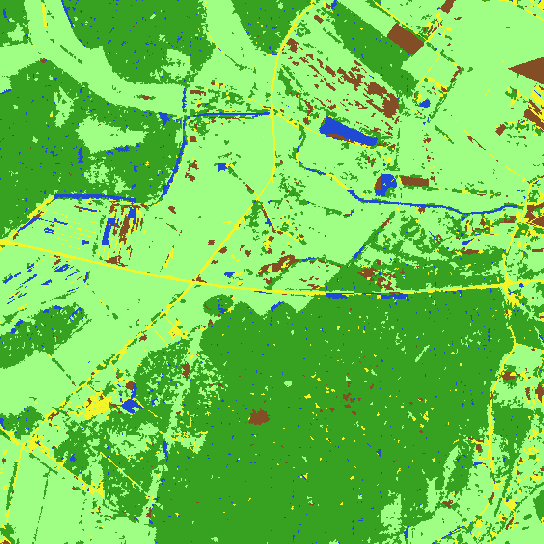
\includegraphics[width=.6\linewidth]{resultNN}
\caption{Klasifikācijas, izmantojot neironu tīklus, rezultāts.}
\label{fig:resultNN}
\end{figure}
\chapter{Validācija un rezultāti}
Pētījumā tika apskatīta krāsu attēlu segmentācijas metode JSEG un citas attēlu segmentācijas metodes, lai noteiktu JSEG metodes priekšrocības un trūkumus salīdzinoši ar citiem krāsu attēlu segmentēšanas algoritmiem. Balstoties uz JSEG metodē iekļautā reģionu apvienošanas algoritma jēgpilnās reģionu grupās vājajiem rezultātiem, tika apskatīta k-tuvāko kaimiņu metode un dziļās apmācības neironu tīkli segmentācijas reģionu klasifikācijai. Lai veiktu zemes pārseguma tipu noteikšanu augstas telpiskās izšķirtspējas tālizpētes datos, tika izstrādāta darbplūsmas abām reģionu klasifikācijas metodēm.\par
Lai pārliecinātos par metodes iespējām un rezultāta pareizību, kā arī, lai veiktu nepieciešamos secinājumus, nepieciešams veikt metodes validāciju. Lai veiktu metodes validāciju, izmantojot programmatūru \textit{QGIS}, tiek izveidots validācijas komplekts. Validācijas komplekts 10 000 $\times$ 10 000 pikseļu  lielam attēlam sastāv no 729 punktiem, kas viens no otra izvietoti 375 pikseļu attālumā režģa formā, kas dabā rezultējas 150 metros. Tabulā \ref{tab:valPunkti} redzama katras klases izplatība un kā jau redzams, visvairāk sastopami tieši koku un zālienu pārseguma tipi, kas izskaidrojams ar to plašo izplatību dabā.
\begin{table}[!ht]
\centering
\caption{Validācijas punktu sadalījums pa klasēm}
\label{tab:valPunkti}
\begin{tabular}{|l|l|l|}
\hline
Klases numurs&Klases nosaukums& Skaits\\ \hline \hline
1&Ūdens&9 \\ \hline
2&Koki & 365\\ \hline
3&Zāliens & 308\\ \hline
4&Lauki & 8\\ \hline
5&Cits & 39\\ \hline
\end{tabular}
\end{table}\par
\begin{figure}[h!]
\centering
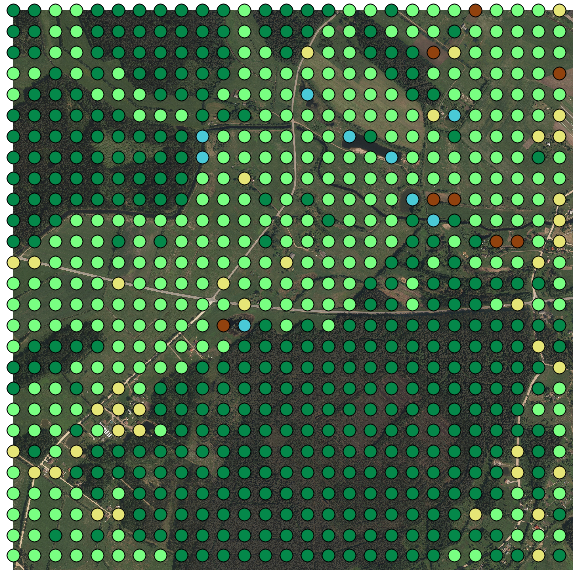
\includegraphics[width=.5\textwidth]{validacija}
\caption{Validācijas komplekts.}
\label{fig:validacija}
\end{figure}\par
Attēlā \ref{fig:validacija} redzams validācijas komplekts un katra punkta atrašanās vieta. Ar tumši zaļo krāsu attēlā apzīmēti punkti, kas pieder klasei "Koki", ar gaiši zaļo krāsu - punkti, kas pieder klasei "Zāliens", ar dzelteno krāsu - punkti, kas pieder klasei "Cits", ar zilo krāsu - punkti, kas pieder klasei "Ūdens", bet ar brūno krāsu - punkti, kas pieder klasei "Lauki". Katram punktam klase ir manuāli piešķirta.\par
Validācija tiek veikta ielasot no faila vērtības, kur vienā kolonnā atrodama punkta "x" koordināta, nākamajā kolonnā punkta "y" koordināta, trešajā kolonnā punkta identifikācijas numurs, kas netiek izmantots, bet pēdējā, punktam piešķirtās klases numurs. Tad interesējošam reģionam tiek izveidota matrica, kur rindu skaits vienāds ar klašu skaitu, bet kolonnu skaits vienāds ar punktu skaitu un, kur vērtības binārā formā reprezentē, vai konkrētais punkts pieder konkrētajai klasei. Tāda pati matrica tiek izveidota arī klasificētajiem reģioniem un pēc tam, izmantojot \textit{MatLab} iebūvēto funkciju \textit{plotconfussion}, tiek iegūta kļūdu matrica, kas parāda, kuri punkti klasificēti pareizi, bet kuri ne.\par
\section{JSEG segmentācijas rezultātu klasifikācijas ar k-tuvāko kaimiņu metodi validācijas rezultāti}Veicot validāciju, izmantojot programmatūru \textit{MatLab}, tās iebūvēto funkciju \textit{plotconfussion} un iepriekš sagatavoto validācijas komplektu, tika iegūta \ref{fig:confMatrix} attēlā redzamā kļūdu matrica. 
\begin{figure}[h!]
\centering
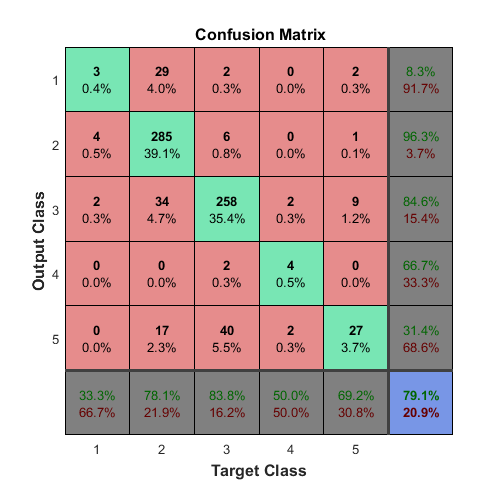
\includegraphics[width=.7\linewidth]{confMatrix}
\caption{Kļūdu matrica klasifikācijai ar k-tuvāko kaimiņu metodi.}
\label{fig:confMatrix}
\end{figure}\par
Metodes precizitāte ir 79,1\%. Visaugstākā precizitāte - 83,8\% ir "zāliena" pārseguma tipa klasei, bet viszemākā precizitāte ir, nosakot reģionu piederību "ūdens" pārseguma tipam - 33,3\%. "Ūdens" pārseguma tips vienlīdz bieži tika sajaukts kā ar "koku" pārseguma tipu, tā "zāliena" pārseguma tipu.\par
"Koku" pārseguma tipam piederošie punkti vienlīdz bieži tika kļūdaini uzskatīti par "ūdens" un "zāliena" klasēm piederošiem punktiem. Tas, ka punkti tika uzskatīti par piederošiem "zāliena" klasei skaidrojams ar plašajām purvainajām teritorijām un jaunaudzēm. Kļūdaini klasificētās "ūdens" teritorijas "koku" klasei piederošiem punktiem skaidrojamas ar vizuālo līdzību starp ūdens teritorijām un ēnām, ko veido koku vainagi.\par
"Zāliena" pārseguma tipam piederošie ortofotokartes punkti 40 gadījumos no 308 tika uzskatīti, ka pieder "citam" zemes pārseguma tipam. Tā kā "cita" pārseguma tipa apmācības datos dominēja reģioni ar ceļa seguma fragmentiem, iespējams, daudzas iebrauktas joslas zālājos sekmēja šādu kļūdainu klasifikāciju.\par 
"Lauku" pārseguma tipa precizitāte ir 50\% un tā vienlīdz bieži tika sajaukta ar "zāliena" un "citu" pārseguma tipu. \par
"Citam" pārseguma tipam atbilstošie punkti visbiežāk kļūdaini tika klasificēti kā piederoši "zāliena" pārseguma tipam, bet tā precizitāte ir 69,2\%\par
Vērojams, ka augstāka precizitāte novērojama tām zemes pārseguma tipa klasēm, kuru apmācībai ne tikai tika izmantots vairāk apmācības datu, bet arī ir vairāk validācijas datu jeb zemes pārseguma tips ir izplatītāks.
\section{JSEG segmentācijas rezultātu klasifikācijas,izmantojot neironu tīklus, validācijas rezultāti}
Veicot validāciju, izmantojot programmatūru \textit{MatLab}, tās iebūvēto funkciju \textit{plotconfussion} un iepriekš sagatavoto validācijas komplektu, tika iegūta \ref{fig:NNconfMatrix} attēlā redzamā kļūdu matrica. 
\begin{figure}[h!]
\centering
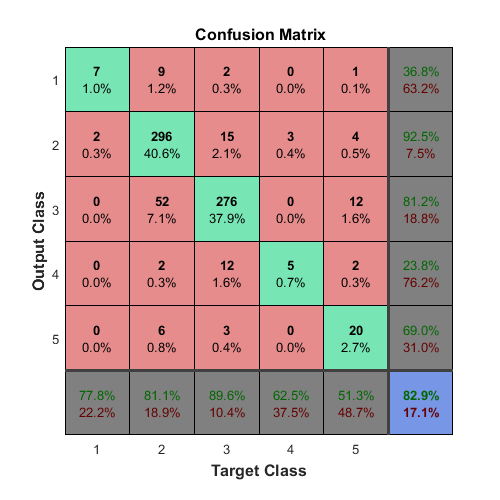
\includegraphics[width=.7\linewidth]{NNconfMatrix}
\caption{Kļūdu matrica klasifikācijai, izmantojot neironu tīklus.}
\label{fig:NNconfMatrix}
\end{figure}\par
Klasificējot reģionus, izmantojot neironu tīklus, tika sasniegta 82,9\% precizitāte. Līdzīgi, kā klasifikācijā, izmantojot k-tuvāko kaimiņu metodi, arī šajā metodē visaugstāko precizitāti - 89,6\% sasniedza to reģionu klasifikācijā, kas atbilst "zāliena" pārseguma tipam. Viszemāko precizitāti - 51,3 \% iespējams novērot nosakot piederību "citam" zemes pārseguma tipam.\par
"Ūdens" pārseguma tipam atbilstošie validācijas punkti tika kļūdaini klasificēti divas reizes kā piederoši "koku" pārseguma tipam, kas gala rezultātā rezultējās 77,8\% precizitātē.\par 
"Koku" pārseguma tipam piederošie punkti visbiežāk - 52 reizes tika kļūdaini uzskatīti par piederošiem "zāliena" pārseguma tipam. Šādu kļūdu iespējams skaidrot ar plašajām purvainajām teritorijām un jaunaudzēm, kas attiecīgajā apgabalā ir plaši izplatītas.\par
"Zāliena" klasei piederošie punkti gandrīz vienādi bieži tika jaukti ar "koku" un "lauku" pārseguma tipiem. "Koku" pārseguma tipa gadījumā kļūda skaidrojama ar ēnām, ko mežu masīvi atstāj zālienā, bet "lauku" pārseguma tipa gadījumā kļūdu iespējams skaidrot ar vizuālo līdzību starp pamestām pļavām un tikko apsētām aramzemēm. \par
"Lauku" pārseguma tipa klasei atbilstošie trīs validācijas punkti no astoņiem kļūdaini tika klasificēti kā piederoši "koku" pārseguma tipam. Šāda kļūda rezultējās 62,5\% precizitātē.\par
"Citam" pārseguma tipam, kam raksturīga viszemākā precizitāte, visbiežāk piederošie punkti tika kļūdaini klasificēti, kā piederoši "zāliena" pārseguma tipam.\par
Līdzīgi, kā klasificējot JSEG segmentācijas rezultātus, izmantojot k-tuvāko kaimiņu metodi, vislabākie rezultāti tika sasniegti tām zemes pārseguma tipu klasēm, kur bija lielākais apmācības datu un validācijas punktu skaits.
\chapter*{Secinājumi un priekšlikumi}
\addcontentsline{toc}{chapter}{Secinājumi un priekšlikumi}
Apkopojot iegūtos rezultātus tiek secināts, ka darba mērķis un tā veikšanai plānotie uzdevumi ir izpildīti. Tāpat autore secina, ka:
\begin{enumerate}
\item JSEG segmentēšanā svarīga loma ir tādiem parametriem, kā attēla kvantizācijā izmantoto krāsu skaitam un attēla apakšapgabala izmēriem, kam tiek pielietots segmentēšanas algoritms. Šo parametru savstarpējā attiecība ietekmē to, cik smalki tiks segmentēts apskatītais attēls. Testējot parametrus, tika secināts, ka labāko rezultātu iespējams iegūt $500 \times 500$ pikseļu lielam apakšapgabalam, izmantojot 12 krāsas attēla kvantizācijā.
\item JSEG segmentēšanas algoritma izpildes laiku iespējams saīsināt, samazinot attēla apakšapgabala izmērus. Viena un tā paša izmēra attēlam, izvēloties 4 reizes vairāk apakšapgabalu izpildes laiks saīsinājās par 17\%.
\item Izvēloties ortofotokartes apakšapgabalu skaitu, jārēķinās, ka lielāks apakšapgabalu skaits garantē arī to, ka ortofotokarte tiks segmentēta vairāk un smalkākos reģionos.
\item Segmentēto reģionu klasifikācijā svarīga loma ir ne tikai tajā, cik labi parauga dati atbilst klasificējamam reģionam, bet arī to skaitam un zemes pārseguma tipa dažādo īpašību reprezentēšanai.
\item Segmentēto reģionu klasifikācija, izmantojot neironu tīklus, uzrādīja par 3,8 \% augstāku precizitāti nekā šo pašu reģionu klasifikācija, izmantojot k-tuvāko kaimiņu metodi.
\item Reģionu deskriptoru vektoru izveidošana, izmantojot reģionu attēlu poligonizāciju programmatūrā \textit{QGIS} un deskriptoru aprēķināšana, izmantojot \textit{Python} skriptu aizņem 100 reizes mazāk laika, kā šī paša rezultāta sasniegšana, izmantojot programmatūru \textit{MatLab}.
\item Reģionu klasifikācija, izmantojot k-tuvāko kaimiņu metodi, aizņem 40 reizes mazāk laika, kā tāda paša apjoma reģionu klasifikācija, izmantojot neironu tīklus. 
\item Pamatojoties uz klasifikācijas metodes izpildes laiku un tā precizitāti, k-tuvāko kaimiņu metode sniedz labākus rezultātus kā reģionu klasificēšana, izmantojot neironu tīklus.
\end{enumerate}\par
Pētījuma gaitā autore izvirza sekojošus priekšlikumus:
\begin{enumerate}
\item Abu pētījumā apskatīto klasifikācijas metožu precizitāti iespējams paaugstināt izvēloties vairāk parauga datu. Tāpat nepieciešams pievērst vairāk uzmanības parauga datu kvalitātei un tam, cik labi tie reprezentē konkrētā pārseguma tipa raksturīgākās īpašības. 
\item Veicot apmācību un sagatavojot parauga datus, parauga datiem vienmērīgi jānoklāj visi zemes pārseguma tipi.
\item Balstoties uz pētījuma apgabalu, vērts ieviest papildus zemes pārseguma tipus, kā piemēram, smilšu segums (lauku ceļi ar grants segumu, karjeri, ūdenstilpju krasti), apdzīvota teritorija (ēkas, viensētas), purvs.
\item Lai uzlabotu skaitļošanas laiku gan segmentācijā, gan klasifikācijā, izmantojot neironu tīklus, nepieciešams palielināt skaitļošanas resursus, izmantojot skaitļošanas klasterus. 
\end{enumerate}
\bibliography{magistraDarbs}{}
\bibliographystyle{plain}
\addcontentsline{toc}{chapter}{Izmantotās literatūras un avotu saraksts}

\chapter*{GALVOJUMS}
\addcontentsline{toc}{chapter}{Galvojums}
\vspace{60pt}
Ar šo es, Katrīna Zvaigzne, galvoju, ka maģistra darbs ir izpildīts patstāvīgi, konsultējoties ar darba vadītāju. No svešiem pirmavotiem ņemtā informācija ir norādīta ar atsaucēm, dati un definējumi ir uzrādīti darbā. Šis darbs tādā vai citādā veidā nav nekad iesniegts nevienai citai pārbaudījumu komisijai. 

\vspace{60pt}
\vspace{1in}

2017.gada \rule{1cm}{0.2pt}.\rule{3cm}{0.2pt} \hspace{3cm}\rule{5cm}{0.2pt}

 \hspace*{11cm}{\raisebox{1em}{(paraksts)}} 
\label{LastPage}
\end{document}
